\documentclass[12pt, titlepage]{article}
\setlength{\headheight}{15pt}

%%%%%%%%%%%%%%%%%%%%%%%%%%%%%%%%%%%%%%%%%%%%%%%%%%%%%%%
%%%% HEADER FILE for CONCRETE MATH LECTURE NOTES %%%%%%
%%%%%%%%%%%%%%%%%%%%%%%%%%%%%%%%%%%%%%%%%%%%%%%%%%%%%%%

%%%%%%%%%%%%%%%%%%%%%%%%%%%%%%%%%%%%%%%%%%%%%%%%%%%%%%%%%%%%%%%%%%%
%% This file is included at the top of every lecture notes file %%%
%% It should ONLY be changed by the instructor %%
%%%%%%%%%%%%%%%%%%%%%%%%%%%%%%%%%%%%%%%%%%%%%%%%%%%%%%%%%%%%%%%%%%%

%%%%%%%%%%%%%%%%%%%%%% package inclusions %%%%%%%%%%%%%%%%%%%%
%\usepackage[
%top=2cm,
%bottom=2cm,
%left=3cm,
%right=2cm,
%headheight=17pt, % as per the warning by fancyhdr
%includehead,includefoot,
%heightrounded, % to avoid spurious underfull messages
%]{geometry} 


\usepackage{amsmath,amssymb,amsfonts}
\usepackage{longtable}
\usepackage{mathtools}
\usepackage{amsthm}
\usepackage{enumerate}
\usepackage{fancyhdr}
\pagestyle{fancy}


%%%%%%%%%%%%%%% theorem style definitions %%%%%%%%%%%%%%%%%%%%%%
\newtheorem{theorem}{Theorem}[section]
%\newtheorem{corollary}{Corollary}[theorem]
%\newtheorem{lemma}[theorem]{Lemma}
\newtheorem*{remark}{Remark}
%\newtheorem{example}{Example}[section]
\newtheorem*{definition}{Definition}


%%%%%%%%%%%%%%%% custom function definitions %%%%%%%%%%%%%%%%%%%%%%%%%
%%%%%%%%%%% as class progresses, this section may be enhanced %%%%%%%%

\def\multiset#1#2{\ensuremath{\left(\kern-.3em\left(\genfrac{}{}{0pt}{}{#1}{#2}\right)
		\kern-.3em\right)}} %%% multiset notation
\newcommand\rf[2]{{#1}^{\overline{#2}}} %%%% rising factorial \rf{x}{m}
\newcommand\ff[2]{{#1}^{\underline{#2}}} %%%%% falling factorial \ff{x}{m}
\newcommand{\Perm}[2]{{}^{#1}\!P_{#2}} % permutation
\newcommand{\half}{\ensuremath{\frac{1}{2}}}
\newcommand{\braces}[1]{\left\{#1\right\}}
\newcommand{\set}[1]{\braces{#1}}
\newcommand{\snb}[2]{\ensuremath{\left(\kern-.3em\left(\genfrac{}{}{0pt}{}{#1}{#2}\right)\kern-.3em\right)}}
\newcommand{\fallingfactorial}[1]{^{\underline{#1}}}
\newcommand{\fallfac}[2]{{#1}^{\underline{#2}}}
\newcommand{\stirlingone}[2]{\genfrac[]{0pt}{1}{#1}{#2}}
\newcommand{\stiri}[2]{\stirlingone{#1}{#2}}
\newcommand{\dstirlingone}[2]{\genfrac[]{0pt}{0}{#1}{#2}}
\newcommand{\dstiri}[2]{\dstirlingone{#1}{#2}}
\newcommand{\stirlingtwo}[2]{\genfrac\{\}{0pt}{1}{#1}{#2}}
\newcommand{\stirii}[2]{\stirlingtwo{#1}{#2}}
\newcommand{\dstirlingtwo}[2]{\genfrac\{\}{0pt}{0}{#1}{#2}}
\newcommand{\dstirii}[2]{\dstirlingtwo{#1}{#2}}
\newcommand{\ol}[1]{\overline{#1}}
%%%%%%%
% book stuff
%%%%%%%%%

\usepackage[twoside,outer=1.5in,inner=2in,bottom=1.5in,top=1.5in,marginpar=2in]{geometry} 
\usepackage{scrextend}
\usepackage{palatino}
\usepackage{multicol}
\usepackage{float}
\usepackage[hidelinks]{hyperref}
\usepackage[nameinlink, capitalise, noabbrev]{cleveref}
%\usepackage{background}
\usepackage{graphicx}
\usepackage{listliketab}

\usepackage{lipsum}
\usepackage{caption}
\usepackage{marginnote}

\reversemarginpar


\usepackage[dvipsnames]{xcolor}
\usepackage{amsthm}
\usepackage{shadethm}

\setlength{\parindent}{0pt}

\newcommand*\Note{%
	\marginnote[\textcolor{blue}{\raggedright{\LARGE ?}\ Note }]{}%
}
\newcommand*\Warn{%
	\marginnote[\textcolor{red}{\raggedright{\LARGE !}\ Warning }]{}%
}
\reversemarginpar

\newcommand{\N}{\mathbb{N}}
\newcommand{\Z}{\mathbb{Z}}
\newcommand{\I}{\mathbb{I}}
\newcommand{\R}{\mathbb{R}}
\newcommand{\Q}{\mathbb{Q}}
\renewcommand{\qed}{\hfill$\blacksquare$}
\let\newproof\proof
\renewenvironment{proof}{\begin{addmargin}[1em]{0em}\begin{newproof}}{\end{newproof}\end{addmargin}\qed}
% \newcommand{\expl}[1]{\text{\hfill[#1]}$}


\newenvironment{lemma}[2][Lemma]{\begin{trivlist}
		\item[\hskip \labelsep {\bfseries #1}\hskip \labelsep {\bfseries #2.}]}{\end{trivlist}}
\newenvironment{problem}[2][Problem]{\begin{trivlist}
		\item[\hskip \labelsep {\bfseries #1}\hskip \labelsep {\bfseries #2.}]}{\end{trivlist}}
\newenvironment{example}[2][Example]{\begin{trivlist}
		\item[\hskip \labelsep {\bfseries #1}\hskip \labelsep{\bfseries #2.}]}{\end{trivlist}}
\newenvironment{solution}{{\noindent \bfseries Solution\hskip 2ex}}{\qed}
\newenvironment{exercise}[2][Exercise]{\begin{trivlist}
		\item[\hskip \labelsep {\bfseries #1}\hskip \labelsep {\bfseries #2.}]}{\end{trivlist}}
\newenvironment{reflection}[2][Reflection]{\begin{trivlist}
		\item[\hskip \labelsep {\bfseries #1}\hskip \labelsep {\bfseries #2.}]}{\end{trivlist}}
\newenvironment{proposition}[2][Proposition]{\begin{trivlist}
		\item[\hskip \labelsep {\bfseries #1}\hskip \labelsep {\bfseries #2.}]}{\end{trivlist}}
\newenvironment{corollary}[2][Corollary]{\begin{trivlist}
		\item[\hskip \labelsep {\bfseries #1}\hskip \labelsep {\bfseries #2.}]}{\end{trivlist}}
% \lhead{\titlestring}
\rhead{Page \thepage}
\cfoot{Concrete Math -- White -- TJHSST}
\renewcommand{\headrulewidth}{0.4pt}
\renewcommand{\footrulewidth}{0.4pt}

% TITLE
\title{Concrete Mathematics}
\author{Dr. Patrick White}
\date{Concrete Mathematics Class Spring 2019} % do not use if [nodate] option enabled

\begin{document}
\maketitle

\tableofcontents

\newpage

\part{Enumeration}

\label{02-0129}
%%%%%%% Lecture Notes Style for Concrete Mathematics %%%%%%%%%%%%%
%%%%%%% Taught by Patrick White, TJHSST %%%%%%%%%%%%%%%%%%%%%%%%%%

%%%% add package inclusions here, if any
%%%%% Define your custom functions and macros here, if any

%%%%%%%%%%%%%%%%%%%% Define the variables below %%%%%%%%%%%%%%%%%%%%%%%%%%%%%%
% \def\titlestring{Introduction to Counting}
% \def\scribestring{Sohom Paul}
% \def\datestring{Tuesday, January, 29 2019}


%%%%%%%%%%%%%%%%%%% Page Headers -- Do Not Change %%%%%%%%%%%%%%%%%%%%%%%%%%%


%%%%%%%%%%%%%%%%% Begin the document %%%%%%%%%%%%%%%%%%%%%%%%%
% \begin{document}
% \thispagestyle{plain}  %% no headers on this page

%%%% Do not change these lines %%%%%
% \noindent
% {\LARGE \textbf{\titlestring}}\\\\
% %
% {\Large Scribe: \scribestring}\\ \\
% {\textbf{Date}: \datestring}


%%%%%%%%%%%%%%%%%%%%%%%%%% YOUR CONTENT GOES HERE %%%%%%%%%%%%%%%%%%%%%%%%%%
% \noindent

\section{Basic Notation}
If $A$ is a set, then we define:

\begin{tabular}{p{1in} p{10cm}}
    $|A|$ or $\#\{A\}$ &  represents the (finite) number of elements in the set, known as the \emph{magnitdue}, \emph{length}, \emph{size}, or \emph{cardinality} of that set\\
    $A \cap B$ & \emph{intersection} (command in \LaTeX\ is \textbackslash cap) \\
    $A \cup B$ & \emph{union} (command in \LaTeX\ is \textbackslash cup) \\
    $\overline{A}$ & \emph{complement}, given by $\{x \mid x \not\in A\}$ \\
    $A \setminus B$ & \emph{minus}, given by $\{x \mid x \in A, x \not\in B\}$; sometimes written as $A-B$ \\
    $x\in A$ & set inclusion ($x$ is an \emph{element} of $A$) \\
    $A \subseteq B$ & A is a \emph{subset} of B ($x\in A \implies x \in B$) \\
    $A \subsetneq B$ & A is a \emph{proper subset} of B ($A\subseteq B, A\neq B$) \\
    $\varnothing$ & empty set \\
    $2^A$ or $\mathcal{P}(A)$ & \emph{power set} of $A$: set of all subsets of $A$, including $A$ and $\varnothing$
\end{tabular}

\section{Counting Strategies}
\subsection{Basic Combinatorics}
\begin{theorem}
$|2^A|=2^{|A|}$
\end{theorem}
\begin{proof} 
We begin with an example.
$$\mathcal{P}(\{1, 2, 3\}) = \{\varnothing, \{1\}, \{2\}, \{3\}, \{1, 2\}, \{1, 3\}, \{2, 3\}, \{1, 2, 3\}\}$$
Notice that the number of subsets is indeed $2^3 = 8$. \\
Many problems in combinatorics are best solved by isomorphic counting; we rephrase the problem into something easier to count. Let us consider the binary functions on $A$,  $f: A \rightarrow \{0, 1\}$. Notice that each $f$ can be uniquely represented with a binary string, which in turn represents a way to make a subset of $A$
\begin{align*}
    001 &\rightarrow f(1) = 0,\, f(2) = 0,\, f(3) = 1 \rightarrow \{3\}\\
    110 &\rightarrow f(1) = 1,\, f(2) = 1,\, f(3) = 0 \rightarrow \{1, 2\}
\end{align*}
Thus, $|2^A|$ is equinumerous to the number of binary numbers of length $|A|$, or $2^{|A|}$.
\end{proof}

\begin{theorem}
If $A \subseteq B$ and $B \subseteq A$, then $A = B$
\end{theorem}
\begin{theorem}[Principle of Inclusion-Exclusion]
$|A\cup B| = |A| + |B| - |A \cap B|$
\end{theorem}
The Principle of Inclusion-Exclusion may be applied repeated to count the cardinality of unions of more than two sets:
$$|A\cup B\cup C| = |A| + |B| + |C| - |AB| - |BC| - |AC| + |ABC|$$
Note that when it's clear what we're talking about, we can abbreviate $A\cap B$ as $AB$.

\begin{problem} \\
Prove that, for $m,n\in\mathbb{N}$ selected uniformly at random $$P(\gcd(m,n)=1) = \frac{6}{\pi^2}$$
\end{problem}
\begin{theorem}[Multiplication Theorem]
Given sets $A_1, A_2, \dots A_n$, the number of ways to select an element from each set is $|A_1||A_2|\dots|A_n|$. 
\end{theorem}
\begin{proof}
Draw a multitree  with root nodes in $A_1$ and let each node $x\in A_i$ have as its children $A_{i+1}$. As you traverse from root to leaf, each decision you make corresponds to a selection from that set, and the number of paths from root to leaf is $|A_1||A_2|\dots|A_n|$.
\end{proof}
\begin{corollary}\\
If $|A| = n$, we can select $k$ of these elements, with repetition, in $n^k$ ways.
\end{corollary}
\begin{corollary}\\
If $|A| = n$, we can select $k$ of these elements, without repetition, in $n(n-1)(n-2)\dots (n-k+1)$ ways.
\end{corollary}
We will notate the above expression as 
$$n(n-1)(n-2)\dots(n-k+1) =\prescript{}{n}{P_k} = \prescript{n}{}{P_k}=n^{\underline{k}}$$
The final notation will be the most commonly used in this class. This is called the ``falling factorial". Similar, we can define a ``rising factorial":
$$n^{\overline{k}}=(n)(n+1)\dots(n+r-1)$$

\begin{problem}[Problem 1]\\
How many passwords with only capital letters or digits contain 8, 9, 10 characters, barring repeated characters?
\\ \emph{Answer:} $36^{\underline{8}}+36^{\underline{9}}+36^{\underline{10}}$
\end{problem}
\begin{problem}[Problem 2]\\
How many passwords with only capital letters or digits containing at least 1 digit and 1 letter contain 8, 9, or 10 characters, barring repeated characters?
\\ \emph{Answer:} $(36^{\underline{8}}+36^{\underline{9}}+36^{\underline{10}}) - (26^{\underline{8}}+26^{\underline{9}}+26^{\underline{10}}) - (10^{\underline{8}}+10^{\underline{9}}+10^{\underline{10}})$
\end{problem}
\begin{problem}[Problem 3]\\
How many passwords with only capital letters or digits contain 8 characters and have capital letters in even-numbered spaces (the 0th position, the 2nd position, and so on), allowing for repitition of characters? \\
\emph{Answer:} $5^4 * 36^4$
\end{problem}

\label{03-0131}
\begin{problem}{4}
    How many divisors does the number 496 have? What about the number 360?
\end{problem}

\begin{solution}
    Consider the prime factorizations of these numbers: 
    \[
        496 = 31 \cdot 2^4  \qquad 360 = 5 \cdot 3^2 \cdot 2^3
    \]
    A divisor of these numbers is created by choosing a possible number of 
    prime factors that divide the original number. For example, a divisor
    of 496 can have either 0 or 1 factors of 31, and anywhere from 0 to 4 
    factors of 2. Then the number of divisors of 496 is $(1 + 1) (4 + 1) = 10$,
    and similarly, the number of divisors of 360 is $(1 + 1)(2 + 1)(3 + 1) = 24$, 
    following from the Multiplication Theorem.
\end{solution}

\begin{problem}{5}
    What are the sum of the divisors of 496 and 360? The ``sum of all divisors''
    function is denoted $\sigma(n)$. 
\end{problem}
\begin{solution}
    Using a modification of the Multiplication Theorem, note that the 
    multiplication operation encodes the idea of ``all possible ways of 
    combining two things.'' As such, if we consider the sum of all of the 
    different prime powers that can appear in any divisor and multiply them
    together, we will create a term with every divisor, added together. For
    instance, the sum of the divisors of 496 is:
    \[
        \sigma(496) = (1 + 31)(1 + 2 + 4  + 8 + 16) = 32 \dot 31 = 992
    \]
    and similarly 
    \[
        \sigma(360) = (1 + 5)(1 + 3 + 9)(1 + 2 + 4 + 8) = 6 \cdot 13 \cdot 15 = 1170.
    \]
\end{solution}

\begin{remark}
    If we consider the sum of all \textit{proper} divisors of a positive 
    integer $n$ ($\sigma(n) - n$), we can classify integers into three categories
    based on how $\sigma(n) - n$ compares to $n$: 
    \begin{itemize}
        \item If $\sigma(n) - n < n$, then $n$ is \textit{deficient}. 
        \item If $\sigma(n) - n > n$, then $n$ is \textit{abundant}.
        \item If $\sigma(n) - n = n$, then $n$ is \textit{perfect}.
    \end{itemize}
    In the example above, note that 360 is abundant and 496 is perfect. 

    Finding perfect numbers is actually an incredibly difficult problem in 
    number theory -- in fact, nobody even knows if there exists perfect
    numbers that are odd! In the even case, though, Euler showed that 
    perfect numbers are of the form $2^{p-1}(2^p - 1)$ if $2^p - 1$ is prime 
    (which requires $p$ itself to be prime also). Primes of the form $2^p - 1$
    are called \textbf{Mersenne primes}, and it is not even known if there
    are infinitely many of these primes! Only 51 Mersenne primes are known 
    to exist as of 2023, so we only know of 51 perfect numbers. 

\end{remark}

\subsection{Quotient Sets}
\begin{problem}\\
Let us count the number of permutations of ``ABCD". There are 24 permutations of this string of length 4 (e.g. ABCD, ABDC, ...). There are also 24 permutations of length 3 (e.g. ABC, ABD, ...) Let define equivalence relationship $p_1 \cong p_2$ if they contain the same letters (e.g. ACB $\cong$ ABC). Define an \emph{equivalence class} $C$ to be such that $p_1, p_2 \in C \implies p_1 \cong p_2$.
How many equivalence classes are there out of the 24 permutations of length 3?
\end{problem}
\begin{solution}
There are 4 equivalence classes. Note the following:
\begin{enumerate}
    \item All equivalence classes are of the size same size, 3!
    \item Different equivalence classes are disjoint
    \item The set of all equivalence classes forms a partition of the set of all $4^{\underline{3}}$ permutations of length 3.
\end{enumerate}
Thus, there are $4^{\underline{3}}/3!$ equivalence classes.
\end{solution} \\ \\
By noticing that equivalence classes are of size $r!$, we can now count \emph{combinations}.
\[
\prescript{}{n}{C_r} = \frac{\prescript{}{n}{P_r}}{r!}
\]
% \end{document}

%%%%%%% Lecture Notes Style for Concrete Mathematics %%%%%%%%%%%%%
%%%%%%% Taught by Patrick White, TJHSST %%%%%%%%%%%%%%%%%%%%%%%%%%

\documentclass[11pt,twosided]{article}
%%%%%%%%%%%%%%%%%%%%%%%%%%%%%%%%%%%%%%%%%%%%%%%%%%%%%%%
%%%% HEADER FILE for CONCRETE MATH LECTURE NOTES %%%%%%
%%%%%%%%%%%%%%%%%%%%%%%%%%%%%%%%%%%%%%%%%%%%%%%%%%%%%%%

%%%%%%%%%%%%%%%%%%%%%%%%%%%%%%%%%%%%%%%%%%%%%%%%%%%%%%%%%%%%%%%%%%%
%% This file is included at the top of every lecture notes file %%%
%% It should ONLY be changed by the instructor %%
%%%%%%%%%%%%%%%%%%%%%%%%%%%%%%%%%%%%%%%%%%%%%%%%%%%%%%%%%%%%%%%%%%%

%%%%%%%%%%%%%%%%%%%%%% package inclusions %%%%%%%%%%%%%%%%%%%%
%\usepackage[
%top=2cm,
%bottom=2cm,
%left=3cm,
%right=2cm,
%headheight=17pt, % as per the warning by fancyhdr
%includehead,includefoot,
%heightrounded, % to avoid spurious underfull messages
%]{geometry} 


\usepackage{amsmath,amssymb,amsfonts}
\usepackage{longtable}
\usepackage{mathtools}
\usepackage{amsthm}
\usepackage{enumerate}
\usepackage{fancyhdr}
\pagestyle{fancy}


%%%%%%%%%%%%%%% theorem style definitions %%%%%%%%%%%%%%%%%%%%%%
\newtheorem{theorem}{Theorem}[section]
%\newtheorem{corollary}{Corollary}[theorem]
%\newtheorem{lemma}[theorem]{Lemma}
\newtheorem*{remark}{Remark}
%\newtheorem{example}{Example}[section]
\newtheorem*{definition}{Definition}


%%%%%%%%%%%%%%%% custom function definitions %%%%%%%%%%%%%%%%%%%%%%%%%
%%%%%%%%%%% as class progresses, this section may be enhanced %%%%%%%%

\def\multiset#1#2{\ensuremath{\left(\kern-.3em\left(\genfrac{}{}{0pt}{}{#1}{#2}\right)
		\kern-.3em\right)}} %%% multiset notation
\newcommand\rf[2]{{#1}^{\overline{#2}}} %%%% rising factorial \rf{x}{m}
\newcommand\ff[2]{{#1}^{\underline{#2}}} %%%%% falling factorial \ff{x}{m}
\newcommand{\Perm}[2]{{}^{#1}\!P_{#2}} % permutation
\newcommand{\half}{\ensuremath{\frac{1}{2}}}
\newcommand{\braces}[1]{\left\{#1\right\}}
\newcommand{\set}[1]{\braces{#1}}
\newcommand{\snb}[2]{\ensuremath{\left(\kern-.3em\left(\genfrac{}{}{0pt}{}{#1}{#2}\right)\kern-.3em\right)}}
\newcommand{\fallingfactorial}[1]{^{\underline{#1}}}
\newcommand{\fallfac}[2]{{#1}^{\underline{#2}}}
\newcommand{\stirlingone}[2]{\genfrac[]{0pt}{1}{#1}{#2}}
\newcommand{\stiri}[2]{\stirlingone{#1}{#2}}
\newcommand{\dstirlingone}[2]{\genfrac[]{0pt}{0}{#1}{#2}}
\newcommand{\dstiri}[2]{\dstirlingone{#1}{#2}}
\newcommand{\stirlingtwo}[2]{\genfrac\{\}{0pt}{1}{#1}{#2}}
\newcommand{\stirii}[2]{\stirlingtwo{#1}{#2}}
\newcommand{\dstirlingtwo}[2]{\genfrac\{\}{0pt}{0}{#1}{#2}}
\newcommand{\dstirii}[2]{\dstirlingtwo{#1}{#2}}
\newcommand{\ol}[1]{\overline{#1}}
%%%%%%%
% book stuff
%%%%%%%%%

\usepackage[twoside,outer=1.5in,inner=2in,bottom=1.5in,top=1.5in,marginpar=2in]{geometry} 
\usepackage{scrextend}
\usepackage{palatino}
\usepackage{multicol}
\usepackage{float}
\usepackage[hidelinks]{hyperref}
\usepackage[nameinlink, capitalise, noabbrev]{cleveref}
%\usepackage{background}
\usepackage{graphicx}
\usepackage{listliketab}

\usepackage{lipsum}
\usepackage{caption}
\usepackage{marginnote}

\reversemarginpar


\usepackage[dvipsnames]{xcolor}
\usepackage{amsthm}
\usepackage{shadethm}

\setlength{\parindent}{0pt}

\newcommand*\Note{%
	\marginnote[\textcolor{blue}{\raggedright{\LARGE ?}\ Note }]{}%
}
\newcommand*\Warn{%
	\marginnote[\textcolor{red}{\raggedright{\LARGE !}\ Warning }]{}%
}
\reversemarginpar

\newcommand{\N}{\mathbb{N}}
\newcommand{\Z}{\mathbb{Z}}
\newcommand{\I}{\mathbb{I}}
\newcommand{\R}{\mathbb{R}}
\newcommand{\Q}{\mathbb{Q}}
\renewcommand{\qed}{\hfill$\blacksquare$}
\let\newproof\proof
\renewenvironment{proof}{\begin{addmargin}[1em]{0em}\begin{newproof}}{\end{newproof}\end{addmargin}\qed}
% \newcommand{\expl}[1]{\text{\hfill[#1]}$}


\newenvironment{lemma}[2][Lemma]{\begin{trivlist}
		\item[\hskip \labelsep {\bfseries #1}\hskip \labelsep {\bfseries #2.}]}{\end{trivlist}}
\newenvironment{problem}[2][Problem]{\begin{trivlist}
		\item[\hskip \labelsep {\bfseries #1}\hskip \labelsep {\bfseries #2.}]}{\end{trivlist}}
\newenvironment{example}[2][Example]{\begin{trivlist}
		\item[\hskip \labelsep {\bfseries #1}\hskip \labelsep{\bfseries #2.}]}{\end{trivlist}}
\newenvironment{solution}{{\noindent \bfseries Solution\hskip 2ex}}{\qed}
\newenvironment{exercise}[2][Exercise]{\begin{trivlist}
		\item[\hskip \labelsep {\bfseries #1}\hskip \labelsep {\bfseries #2.}]}{\end{trivlist}}
\newenvironment{reflection}[2][Reflection]{\begin{trivlist}
		\item[\hskip \labelsep {\bfseries #1}\hskip \labelsep {\bfseries #2.}]}{\end{trivlist}}
\newenvironment{proposition}[2][Proposition]{\begin{trivlist}
		\item[\hskip \labelsep {\bfseries #1}\hskip \labelsep {\bfseries #2.}]}{\end{trivlist}}
\newenvironment{corollary}[2][Corollary]{\begin{trivlist}
		\item[\hskip \labelsep {\bfseries #1}\hskip \labelsep {\bfseries #2.}]}{\end{trivlist}}

%%%% add package inclusions here, if any
\usepackage{enumerate}

%%%%% Define your custom functions and macros here, if any

\newcommand{\Perm}[2]{{}^{#1}\!P_{#2}}%

%%%%%%%%%%%%%%%%%%%% Define the variables below %%%%%%%%%%%%%%%%%%%%%%%%%%%%%%
\def\titlestring{Day 4: More Counting}
\def\scribestring{Caroline Jin}
\def\datestring{Tuesday, February, 5 2019}


%%%%%%%%%%%%%%%%%%% Page Headers -- Do Not Change %%%%%%%%%%%%%%%%%%%%%%%%%%%
\lhead{\titlestring}
\rhead{Page \thepage}
\cfoot{Concrete Math -- White -- TJHSST}
\renewcommand{\headrulewidth}{0.4pt}
\renewcommand{\footrulewidth}{0.4pt}

%%%%%%%%%%%%%%%%% Begin the document %%%%%%%%%%%%%%%%%%%%%%%%%
\begin{document}
\thispagestyle{plain}  %% no headers on this page

%%%% Do not change these lines %%%%%
\noindent
{\LARGE \textbf{\titlestring}}\\\\
%
{\Large Scribe: \scribestring}\\ \\
{\textbf{Date}: \datestring}


%%%%%%%%%%%%%%%%%%%%%%%%%% YOUR CONTENT GOES HERE %%%%%%%%%%%%%%%%%%%%%%%%%%
\noindent

\section{Partitions}
    A \textit{partition} of a set $S$ is a subset of $S_1, ... S_k$ such that
\begin{enumerate}[(i)]
        \item $\bigcup\limits_{i=1}^{k} S_{i}$. The subsets `cover' the set $S$
        \item $S_i 	\cap S_j = \varnothing$. The subsets are pairwise disjoint.
        \item $S_i \neq \varnothing$
\end{enumerate}

\begin{problem}
    1 Let $S$ be the set of all integers composed of digits in $\{1, 3, 5, 7\}$ at most one.
    
    \begin{enumerate}[(i)]
        \item Find $|S|$
        \item $\sum\limits_{x \in S} x$
    \end{enumerate}
\end{problem}

\begin{solution}
    \begin{enumerate}[(i)]
        \item Let $S = S_1 \cup S_2 \cup S_3 \cup S_4$ where $S_1$ is the number of one digit numbers, $S_2$ is the number of two-digit numbers, and so on. \\
            \[|S_1| = \Perm{4}{1} = 4\]
            \[|S_2| = \Perm{4}{2} = 12\]
            \[|S_3| = \Perm{4}{3} = 24\]
            \[|S_4| = \Perm{4}{4} = 24\]
            \[|S| = |S_1| + |S_2| + |S_3| + |S_4| = \boxed{64}\]
        \item Let $\alpha = \alpha_1 + 10\alpha_2 + 100\alpha_3 + 1000\alpha_4$ where $\alpha_1$ is the sum of all units digits of all numbers in $S$, $\alpha_2$ is the sum of all the tens digits of all the numbers, and so on. We will find the value of $\alpha_1$ using the following: 
        \begin{align*}
            &S_1 \rightarrow s_1 = (1+3+5+7)\\
            &S_2 \rightarrow s_2 = (1+3+5+7)\times (3)\\
            &S_3 \rightarrow s_3 = (1+3+5+7)\times (3\times2)\\
            &S_4 \rightarrow s_4 = (1+3+5+7)\times (3\times2\times1)\\
            \hline
            &\alpha_1 = 16 \times (1+3+6+6) = 256
        \end{align*}
        Note that $\alpha_2$ is the sum of the same values, excluding $s_1$ as $S_1$ is the set of only one digit numbers. $\alpha_3$ is the sum of the same values as $\alpha_2$, excluding $s_2$ as $S_2$ is the set of only two digit numbers, and so on.
        \begin{align*}
            &\alpha_2 = \alpha_1 - s_1 = 240\\
            &\alpha_3 = \alpha_2 - s_2 = 192\\
            &\alpha_4 = \alpha_3 - s_3 = 96\\
        \end{align*}
        Thus, $\alpha = \alpha_1 + 10\alpha_2 + 100\alpha_3 + 1000\alpha_4 = \boxed{117,856}$
        \\\\
        An easier solution is the following:
        \begin{align*}
            &1 + 3 + 5 + 7 = (1 + 7) + (3 + 5) = 8(\frac{4}{2}) = 16\\
            &13 + ... + 75 = (13 + 75) + ... + (35 + 53) = 88(\frac{12}{2}) = 528\\
            &\text{etc}
        \end{align*}
        Since each $x \in S_i$ pairs with $ \bar{x} \in S_i$ to sum to $88...8$. We find $\alpha = 8\frac{|S_1|}{2} + 88\frac{|S_2|}{2} + 888\frac{|S_3|}{2} + 8888\frac{|S_4|}{2} = \boxed{117,856}$
    \end{enumerate}
    
\end{solution}

\section{Cyclic Permutation}

Consider the set $T$ of 3 permutations of $(s_1, s_2, s_3, s_4)$ or $(1, 2, 3, 4)$. We know that $T = \{ 123, 132, 234, 214, ... \}$ and $|T| = P(4, 3) = 24$.\\

We define $x \cong y \iff x + y $ are cyclically equivalently 

\begin{problem}
    1 Given $123 \cong x$, how many solutions are there for $x \in T$?
\end{problem}

\begin{solution}
    The $x$ values are 123, 231, 312, so there are \boxed{3} solutions. Thus, we see any sequence of length $n \cong n$ sequences
\end{solution}

\begin{theorem}
    If $Q(n, r)$ is the number of cyclic permutations of length $r$ from a set of $n$ elements, $Q(n, r) = \frac{P(n, r)}{r}$.
\end{theorem}

\begin{theorem}
    There are (n-1)! ways to seat n people around a round table.
\end{theorem}

\begin{proof}
    Each ordering $\cong n$ orderings. Thus, $\frac{n!}{n} = (n-1)!$
\end{proof}

\begin{problem}
    2 There are 5 boys and 3 girls seated around a round table.
    \begin{enumerate}[(i)]
        \item There are no restrictions.
        \item $B_1$ and $G_1$ are not adjacent
        \item No girls are adjacent to other girls
    \end{enumerate}
\end{problem}

\begin{solution}
    \begin{enumerate}[(i)]
        \item Using theorem 2.1, there are \boxed{7!} ways.
        \item We first place $B_1$ in any of the 7 seats and set $B_1$ as our reference point. There are then 5 places for $G_1$ to sit not adjacent to $B_1$ and 6! ways for the remaining 6 people to sit. The total number of ways if $\boxed{6! \cdot 5}$. We can also consider the number of ways for $B_1$ and $G_1$ to sit next to each other, which is $2 \cdot 6!$. Subtracting that from arranging without restrictions, the total number of ways is $\boxed{7! - 2 \cdot 6!}$ 
        \item We first arrange all the 5 boys, which is $4!$ ways. There are 5 spaces between each boy, so we can choose 3 of the seats and then arrange the 3 girls, $\binom{5}{3} \cdot 3!$. The total number of ways is $\boxed{4! \cdot \binom{5}{3} \cdot 3!}$
    \end{enumerate}
\end{solution}
\section{Recursion}
\begin{exercise}
    1 Find the recursive definition of $P(n,r)$.
\end{exercise}

\begin{solution}
    We know that the closed form of $P(n,r) = \frac{n!}{(n-r)!}$. Our goal is to define $P(n, r) = f(P(<n, <r))$.\\
    Let $S = \{s_1, ..., s_n\}$, r be given $0 \leq r \leq n$, and $T$ be the set of all r-permutations of $S$.
    \noindent
    We can partition $T$ into $T = T_1 \cup T_2$ where
    \begin{align*}
        &t = T_1 \Leftrightarrow s_1 \notin t \text{ (no $s_1$)}\\
        &t = T_2 \Leftrightarrow s_1 \in t \text{ (yes $s_1$)}
    \end{align*}
    We can find the $|T_1|$ in terms of $P(\leq n, \leq r)$
    \begin{align*}
        &|T_1| = P(n-1, r)\\
        &|T_2| = r \cdot P(n-1, r-1) 
    \end{align*}
    For $|T_2|$, we can order $r-1$ elements from $\{s_2, ..., s_n \}$ and place $s_1$ in any of the $r$ locations. Thus, $\boxed{P(n,r) = P(n-1,r) + r \cdot P(n-1, r-1)}$
\end{solution}

\begin{exercise}
    2 Find a recursive definition of $C(n, r)$
\end{exercise}

\begin{solution}
    Again, let $T$ be the subset of $S = \{s_1, ... , s_n\}$ of size $r$.\\
    To find $|T|$, let $T = T_1 \cup T_2$ where $T_1$ has no set containing $s_1$ and $T_2$ has every set containing $s_1$.
    \begin{align*}
        &|T_1| = C(n-1, r) \text{ we can choose $r$ from $s_2, ... s_n$}\\
        &|T_2| = C(n-1, r-1) \text{ we choose $r-1$ from $s_2, ... s_n$ and add in $s_1$}
    \end{align*}
    Thus, $\boxed{C(n, r) = C(n-1, r) + C(n-1, r-1)}$
\end{solution}

\begin{problem}
    1 Given $2n$ tennis players. How many ways are there to arrange $n$ games/pairings?
\end{problem}

\begin{solution}
    There are several solutions to this problem:
    \begin{enumerate}
        \item We can match $P_1$ with another $2n - 1$ players. For the next player $P_2$ who hasn't been matched, we can choose $2n - 3$ players, and so on. The solution is just $(2n-1)(2n-3)...(1) = \boxed{(2n-1)!!}$
        \item We can choose each pair and divide by $n!$ to remove the ordering of the pairs. There are $\boxed{\frac{\binom{2n}{n}\binom{2n-2}{2} ... \binom{2}{2}}{n!}}$ ways. 
        \item We can permute all $2n$ players and divide by $n!$ (the number of ways to order the game doesn't matter) and $2^n$ (the order of the partners doesn't matter). There are $\boxed{\frac{(2n)!}{n!2^n}}$
    \end{enumerate}

\end{solution}
\end{document}


%%%%%%% Lecture Notes Style for Concrete Mathematics %%%%%%%%%%%%%
%%%%%%% Taught by Patrick White, TJHSST %%%%%%%%%%%%%%%%%%%%%%%%%%

\documentclass[11pt,twosided]{article}
%%%%%%%%%%%%%%%%%%%%%%%%%%%%%%%%%%%%%%%%%%%%%%%%%%%%%%%
%%%% HEADER FILE for CONCRETE MATH LECTURE NOTES %%%%%%
%%%%%%%%%%%%%%%%%%%%%%%%%%%%%%%%%%%%%%%%%%%%%%%%%%%%%%%

%%%%%%%%%%%%%%%%%%%%%%%%%%%%%%%%%%%%%%%%%%%%%%%%%%%%%%%%%%%%%%%%%%%
%% This file is included at the top of every lecture notes file %%%
%% It should ONLY be changed by the instructor %%
%%%%%%%%%%%%%%%%%%%%%%%%%%%%%%%%%%%%%%%%%%%%%%%%%%%%%%%%%%%%%%%%%%%

%%%%%%%%%%%%%%%%%%%%%% package inclusions %%%%%%%%%%%%%%%%%%%%
%\usepackage[
%top=2cm,
%bottom=2cm,
%left=3cm,
%right=2cm,
%headheight=17pt, % as per the warning by fancyhdr
%includehead,includefoot,
%heightrounded, % to avoid spurious underfull messages
%]{geometry} 


\usepackage{amsmath,amssymb,amsfonts}
\usepackage{longtable}
\usepackage{mathtools}
\usepackage{amsthm}
\usepackage{enumerate}
\usepackage{fancyhdr}
\pagestyle{fancy}


%%%%%%%%%%%%%%% theorem style definitions %%%%%%%%%%%%%%%%%%%%%%
\newtheorem{theorem}{Theorem}[section]
%\newtheorem{corollary}{Corollary}[theorem]
%\newtheorem{lemma}[theorem]{Lemma}
\newtheorem*{remark}{Remark}
%\newtheorem{example}{Example}[section]
\newtheorem*{definition}{Definition}


%%%%%%%%%%%%%%%% custom function definitions %%%%%%%%%%%%%%%%%%%%%%%%%
%%%%%%%%%%% as class progresses, this section may be enhanced %%%%%%%%

\def\multiset#1#2{\ensuremath{\left(\kern-.3em\left(\genfrac{}{}{0pt}{}{#1}{#2}\right)
		\kern-.3em\right)}} %%% multiset notation
\newcommand\rf[2]{{#1}^{\overline{#2}}} %%%% rising factorial \rf{x}{m}
\newcommand\ff[2]{{#1}^{\underline{#2}}} %%%%% falling factorial \ff{x}{m}
\newcommand{\Perm}[2]{{}^{#1}\!P_{#2}} % permutation
\newcommand{\half}{\ensuremath{\frac{1}{2}}}
\newcommand{\braces}[1]{\left\{#1\right\}}
\newcommand{\set}[1]{\braces{#1}}
\newcommand{\snb}[2]{\ensuremath{\left(\kern-.3em\left(\genfrac{}{}{0pt}{}{#1}{#2}\right)\kern-.3em\right)}}
\newcommand{\fallingfactorial}[1]{^{\underline{#1}}}
\newcommand{\fallfac}[2]{{#1}^{\underline{#2}}}
\newcommand{\stirlingone}[2]{\genfrac[]{0pt}{1}{#1}{#2}}
\newcommand{\stiri}[2]{\stirlingone{#1}{#2}}
\newcommand{\dstirlingone}[2]{\genfrac[]{0pt}{0}{#1}{#2}}
\newcommand{\dstiri}[2]{\dstirlingone{#1}{#2}}
\newcommand{\stirlingtwo}[2]{\genfrac\{\}{0pt}{1}{#1}{#2}}
\newcommand{\stirii}[2]{\stirlingtwo{#1}{#2}}
\newcommand{\dstirlingtwo}[2]{\genfrac\{\}{0pt}{0}{#1}{#2}}
\newcommand{\dstirii}[2]{\dstirlingtwo{#1}{#2}}
\newcommand{\ol}[1]{\overline{#1}}
%%%%%%%
% book stuff
%%%%%%%%%

\usepackage[twoside,outer=1.5in,inner=2in,bottom=1.5in,top=1.5in,marginpar=2in]{geometry} 
\usepackage{scrextend}
\usepackage{palatino}
\usepackage{multicol}
\usepackage{float}
\usepackage[hidelinks]{hyperref}
\usepackage[nameinlink, capitalise, noabbrev]{cleveref}
%\usepackage{background}
\usepackage{graphicx}
\usepackage{listliketab}

\usepackage{lipsum}
\usepackage{caption}
\usepackage{marginnote}

\reversemarginpar


\usepackage[dvipsnames]{xcolor}
\usepackage{amsthm}
\usepackage{shadethm}

\setlength{\parindent}{0pt}

\newcommand*\Note{%
	\marginnote[\textcolor{blue}{\raggedright{\LARGE ?}\ Note }]{}%
}
\newcommand*\Warn{%
	\marginnote[\textcolor{red}{\raggedright{\LARGE !}\ Warning }]{}%
}
\reversemarginpar

\newcommand{\N}{\mathbb{N}}
\newcommand{\Z}{\mathbb{Z}}
\newcommand{\I}{\mathbb{I}}
\newcommand{\R}{\mathbb{R}}
\newcommand{\Q}{\mathbb{Q}}
\renewcommand{\qed}{\hfill$\blacksquare$}
\let\newproof\proof
\renewenvironment{proof}{\begin{addmargin}[1em]{0em}\begin{newproof}}{\end{newproof}\end{addmargin}\qed}
% \newcommand{\expl}[1]{\text{\hfill[#1]}$}


\newenvironment{lemma}[2][Lemma]{\begin{trivlist}
		\item[\hskip \labelsep {\bfseries #1}\hskip \labelsep {\bfseries #2.}]}{\end{trivlist}}
\newenvironment{problem}[2][Problem]{\begin{trivlist}
		\item[\hskip \labelsep {\bfseries #1}\hskip \labelsep {\bfseries #2.}]}{\end{trivlist}}
\newenvironment{example}[2][Example]{\begin{trivlist}
		\item[\hskip \labelsep {\bfseries #1}\hskip \labelsep{\bfseries #2.}]}{\end{trivlist}}
\newenvironment{solution}{{\noindent \bfseries Solution\hskip 2ex}}{\qed}
\newenvironment{exercise}[2][Exercise]{\begin{trivlist}
		\item[\hskip \labelsep {\bfseries #1}\hskip \labelsep {\bfseries #2.}]}{\end{trivlist}}
\newenvironment{reflection}[2][Reflection]{\begin{trivlist}
		\item[\hskip \labelsep {\bfseries #1}\hskip \labelsep {\bfseries #2.}]}{\end{trivlist}}
\newenvironment{proposition}[2][Proposition]{\begin{trivlist}
		\item[\hskip \labelsep {\bfseries #1}\hskip \labelsep {\bfseries #2.}]}{\end{trivlist}}
\newenvironment{corollary}[2][Corollary]{\begin{trivlist}
		\item[\hskip \labelsep {\bfseries #1}\hskip \labelsep {\bfseries #2.}]}{\end{trivlist}}

%%%% add package inclusions here, if any
\usepackage{amsmath, amssymb, amsthm, amsfonts}
\usepackage{mathtools}
\usepackage{nccmath}

%%%%% Define your custom functions and macros here, if any
\newcommand{\half}{\ensuremath{\frac{1}{2}}}
\DeclarePairedDelimiter{\braces}{\{}{\}}
\newcommand{\set}{\braces}
\newcommand{\snb}[2]{\left(\binom{#1}{#2}\right)}
%%%%%%%%%%%%%%%%%%%% Define the variables below %%%%%%%%%%%%%%%%%%%%%%%%%%%%%%
\def\titlestring{Combinations, Multisets, Binomial Expansions}
\def\scribestring{Bryan Lu}
\def\datestring{February 7, 2019}


%%%%%%%%%%%%%%%%%%% Page Headers -- Do Not Change %%%%%%%%%%%%%%%%%%%%%%%%%%%
\lhead{\titlestring}
\rhead{Page \thepage}
\cfoot{Concrete Math -- White -- TJHSST}
\renewcommand{\headrulewidth}{0.4pt}
\renewcommand{\footrulewidth}{0.4pt}

%%%%%%%%%%%%%%%%% Begin the document %%%%%%%%%%%%%%%%%%%%%%%%%
\begin{document}
\thispagestyle{plain}  %% no headers on this page

%%%% Do not change these lines %%%%%
\noindent
{\LARGE \textbf{\titlestring}}\\\\
%
{\Large Scribe: \scribestring}\\ \\
{\textbf{Date}: \datestring}


%%%%%%%%%%%%%%%%%%%%%%%%%% YOUR CONTENT GOES HERE %%%%%%%%%%%%%%%%%%%%%%%%%%
\noindent

%\section{Revisiting Cyclic Permutations}
%\begin{problem}{1}
%How many ways are there to arrange 5 boys and 3 girls around a table such that no girls are adjacent?
%\end{problem}
%Consider the following "bogus solution":
%\begin{solution}
%	Arrange the boys in a line in 5! ways, choose three of the boys to put girls to the left of, and arrange the girls in 3! ways. \textit{We then divide by 8 in order to account for the cyclicity of the table.}
%\end{solution}
%\newline
%Recall, however, the \textbf{reason} we divided by $8$ to begin with is to divide by the size of each of the equivalence groups in the original problem when arranging people around the table. There are \textbf{not} $8$ elements in each of these equivalence groups - cyclical arrangements with a girl on the very right is not part of set that we counted. In fact, there are only $5$. 


\section{Points in the Plane}
Here is a difficult but interesting problem from the International Mathematical Olympiad that uses the counting techniques we have encountered thus far, but in a creative manner:
\begin{problem}{1} 
\textbf{(IMO 1989/3)} Given $n, k \in \Z^+$, let $S$ be a set of $n$ points in the plane such that no three points of $S$ are collinear, and for any point $P$ of $S$ there are at least $k$ points of $S$ equidistant from $P$. Prove that 
\[
	k < \frac{1}{2} + \sqrt{2n}
\]
\end{problem}

\begin{proof}
We will count the edges between all pairs of points. One way to do so is simply choose any two of the points, which can be done in $\binom{n}{2}$ ways. \\
	The other way we can do so is by counting edges among the points equidistant from a point $P$. We can compute all pairs of edges between these equidistant points, which gives at least $\binom{k}{2}$ edges. Across all points, this gives at least $n\binom{k}{2}$. However, we have overcounted - notice that each edge can represent at a maximum one intersection between the two circles representing equidistant sets of points around each point. If this edge was the intersection of three or more of these circles, this would give at least three points in $S$ as collinear, which is forbidden. This means that we have overcounted by at most $\binom{n}{2}$. This method of counting may not have accounted for all the edges, so all in all we obtain the inequality 
\[
	\binom{n}{2} \geq n\binom{k}{2} - \binom{n}{2}
\]
Expanding, we have: 
\[
	2\cdot \frac{n(n-1)}{2} \geq \frac{nk(k-1)}{2}
\] 
\[
	n - 1 \geq \frac{k^2 - k}{2}
\]
\[
	n \geq 1 + \frac{4k^2 - 4k}{8} > \frac{4k^2 - 4k + 1}{8}
\]	
\[
	8n > (2k-1)^2
\]
\[
	2\sqrt{2n} > 2k - 1
\]
\[
	k < \half + \sqrt{2n}
\]
as desired.
\end{proof}

\section{Binomial Coefficients}
Recall we derived a recursive definition of combinations (ie. binomial coefficients) in the last lecture: 
\[
	\binom{n}{k} = \binom{n-1}{k} + \binom{n-1}{k-1}
\]
This is also known as \textbf{Pascal's Identity}.\\
We now prove the famed \textbf{Binomial Theorem}: 
\[
	(x+y)^n = \sum_{k=0}^n \binom{n}{k} x^k y^{n-k}
\]
While proving this fact, we will extend the definition of the combination (or binomial coefficient) as follows:
\[
	\binom{n}{k} = \begin{cases} 
      \frac{\ff{n}{k}}{k!} & 0 \leq k \leq n \\
      0 & k > n, k < 0
   \end{cases}
\]
We will prove this in two ways - first by induction and then by a simple combinatorial argument. 
\begin{proof}[Proof 1.]
	First, let us consider the trivial base case for $n=0$, for which $(x+y)^0 = 1$ which is easily true, as $\binom{0}{0} = 1$.  \\
	For the inductive step, we can consider $(x+y)^{n+1}$ as $(x+y)(x+y)^n$, and apply the Binomial Theorem to the $(x+y)^n$ term. We expand: 
\begin{align*}
(x+y)(x+y)^n &= (x+y) \sum_{k=0}^n \binom{n}{k} x^k y^{n-k} \\
&= \sum_{k=0}^n \binom{n}{k} x^{k+1} y^{n-k} + \sum_{k=0}^n \binom{n}{k} x^k y^{n+1-k} \\
&= \sum_{k=1}^{n+1} \binom{n}{k-1} x^{k} y^{n+1-k} + \sum_{k=0}^n \binom{n}{k} x^k y^{n+1-k} 
\end{align*}
where we shift the indices of the first sum back so the exponents of the $x$ and $y$ terms match up. We will now extend the bounds of each of the sums by one in order to combine them together into one sum - this is legal, as the terms that we are adding are zero by our extended definition of the binomial coefficient. 
\[
	\sum_{k=0}^{n+1} \binom{n}{k-1} x^{k} y^{n+1-k} + \sum_{k=0}^{n+1} \binom{n}{k} x^k y^{n+1-k} 
\]
Now we finish using Pascal's Identity:
\[
	\sum_{k=0}^{n+1} \left(\binom{n}{k-1} + \binom{n}{k}\right) x^{k} y^{n-k} = \sum_{k=0}^{n+1} \binom{n+1}{k} x^{k} y^{n-k} 
\]
\end{proof}
\begin{proof}[Proof 2.]
	We can write the product $(x+y)^n$ out explicitly:
\[
	(x+y)^n = \overbrace{(x+y)(x+y)\ldots (x+y)}^n
\]
Notice that the term $x^k y^{n-k}$ appears $\binom{n}{k}$ times, which immediately implies the desired as we sum over all possible $k$. 
\end{proof}
\begin{reflection}{A}
Notice how much cleaner the combinatorial argument was! We will appeal to such arguments again and again as the course progresses.
\end{reflection}
What if we want to expand something like $(1-x)^{\frac{1}{2}}$ binomially? This forces us to define binomial coefficients when the top argument is a real $\alpha$ - and furthermore, we have to define them in such a way so that it doesn't involve factorials of $\alpha$ (which aren't well defined). We can define as follows for $\binom{\alpha}{n}$ if $n$ is an integer, but $\alpha$ can be any real: 
\[
	\binom{\alpha}{n} =  \frac{\alpha (\alpha - 1) (\alpha - 2) \ldots (\alpha - n + 1)}{n! } = \frac{\ff{\alpha}{n}}{n!}
\]
Once this is done, we can simply apply the Binomial Theorem, which turns out still to be true with this definition, except the sum does not terminate (left to the reader as an exercise): 
\begin{align*}
(1-x)^{\frac{1}{2}} &= \sum_{k=0}^{\infty} \binom{\half}{k} (-x)^k \\
&= 1 + \frac{\half}{1!}(-x)^1 + \frac{\half \left(-\half \right)}{2!} (-x)^2 + \frac{\half \left(-\half \right) \left(-\frac{3}{2} \right)}{3!} (-x)^3  + \ldots 
\end{align*}
\[
\implies (1-x)^{\frac{1}{2}} = 1 - \sum_{n=0}^{\infty} \frac{(2n-1)!!}{(n+1)!2^{n+1}} x^{n+1}	
\]
where we define $(-1)!! = 1$. \\
Recall we had this double factorial last class, and in fact we showed that $(2n-1)!! = \frac{(2n)!}{2^n n!}$ by solving the same combinatorial problem of creating games in a tournament. Applying this, we obtain
\begin{align*}
(1-x)^{\frac{1}{2}} &= 1 - \sum_{n=0}^{\infty} \frac{(2n)!}{(n!)(n+1)!2^{n+1}2^n} x^{n+1}	\\
&= 1 - \frac{1}{2}\sum_{n=0}^{\infty} \frac{(2n)!}{(n!)(n+1)! 4^{n}} x^{n+1} \\
&= 1 - \frac{1}{2}\sum_{n=0}^{\infty} \frac{(2n)!}{(n!)^2(n+1) 4^{n}} x^{n+1}\\
&=  1 - \frac{1}{2}\sum_{n=0}^{\infty} \binom{2n}{n} \frac{1}{n+1}\cdot \frac{1}{4^n} x^{n+1}
\end{align*}
\begin{remark}
The term $\binom{2n}{n} \frac{1}{n+1}$ is the $n$th \textbf{Catalan number}. We will see these numbers again in the near future. 
\end{remark}


\section{Multisets and Problems with Repetition}
We will now start to look at problems where we can have repetition of elements. Consider the following problems: 
\begin{problem}{2}
Given the elements of the set $\set{ a, b, c, d }$, how many ways are there to construct a sequence of length 7 with repetition allowed?  
\end{problem}
\begin{proof}[Solution.]
For each element in the sequence, we can choose any element in the set, giving $\boxed{4^7}$ possibilities.
\end{proof}
\begin{problem}{3}
Given the multiset $\set{ 3\cdot a, 2\cdot b, 5 \cdot c }$, how many unique sequences are there that use all the letters once?
\end{problem}
\begin{proof}[Solution.]
If we first label the $a$s, $b$s, and $c$s so that they are distinguishable, we can arrange all the letters in $10!$ ways to begin with. However, since all of the $a$s are indistinguishable, permuting the order of the labeled $a$s produces an equivalent arrangement - so we must divide by a factor of $3!$. We must do the same thing for the $b$s and $c$s, giving $\boxed{\frac{10!}{3! 2! 5!}}$ sequences. 
\end{proof}
\begin{problem}{4}
Given the multiset $\set{ \infty \cdot a, \infty \cdot b, \infty \cdot c, \infty \cdot d }$, how many ways can one choose a sub-multiset of size $7$? 
\end{problem}
\begin{proof}[Solution.]
Notice that we only care about the quantities of each of the letters $a, b, c, d$, so we can consider the equivalent problem of finding the number of positive-integer solutions to the equation $w + x + y + z = 7$. This can be counted by considering the isomorphic problem of counting binary strings of length 10 with three 1s. To see why this problem is the same as counting solutions to the equation, notice that for every such binary string, we can let the number of $0$s to the left of the first 1 be the value of $w$, the number of $0$s between the first and second 1s be the value of $x$, etc. This uniquely maps this binary string to a solution to this Diophantine equation, and similarly every solution to the equation gives a binary string. We can count the strings easily - there are  $\boxed{\binom{10}{3}}$ of these strings, which is the answer to the original problem as well.
\end{proof}
\newline
We can generalize this last problem: with the same reasoning, we find the number of ways to build a size-$r$ multiset from $n$ possible elements is $\binom{n-1+r}{n-1} = \binom{n-1+r}{r}$. \\
We now define some additional notation for these kinds of problems: 
\begin{itemize}
\item We denote the number of multisets into a sequence as a \textit{multinomial coefficient}:
\[
	\binom{n}{r_1, r_2, \ldots r_k} = \frac{n!}{r_1! r_2! \ldots r_k!}
\]
where $n = \sum_i r_i$. 
\item The number of multisets of length $r$ constructed from $n$ possible elements (colloquially known as the \textit{stars and bars} problem) is denoted as 
\[
	\snb{n}{r} = \binom{n-1+r}{n-1} = \binom{n-1+r}{r}
\]
For example, $\snb{3}{7} = \binom{3-1+7}{2} = \binom{9}{2} = 36$. Note that unlike binomial coeffients, $n$ need not be less than $r$! 
\end{itemize}






\end{document}


\label{08-0219}
%%%%%%% Lecture Notes Style for Concrete Mathematics %%%%%%%%%%%%%
%%%%%%% Taught by Patrick White, TJHSST %%%%%%%%%%%%%%%%%%%%%%%%%%

% \documentclass[11pt,twosided]{article}
% %%%%%%%%%%%%%%%%%%%%%%%%%%%%%%%%%%%%%%%%%%%%%%%%%%%%%%%
%%%% HEADER FILE for CONCRETE MATH LECTURE NOTES %%%%%%
%%%%%%%%%%%%%%%%%%%%%%%%%%%%%%%%%%%%%%%%%%%%%%%%%%%%%%%

%%%%%%%%%%%%%%%%%%%%%%%%%%%%%%%%%%%%%%%%%%%%%%%%%%%%%%%%%%%%%%%%%%%
%% This file is included at the top of every lecture notes file %%%
%% It should ONLY be changed by the instructor %%
%%%%%%%%%%%%%%%%%%%%%%%%%%%%%%%%%%%%%%%%%%%%%%%%%%%%%%%%%%%%%%%%%%%

%%%%%%%%%%%%%%%%%%%%%% package inclusions %%%%%%%%%%%%%%%%%%%%
%\usepackage[
%top=2cm,
%bottom=2cm,
%left=3cm,
%right=2cm,
%headheight=17pt, % as per the warning by fancyhdr
%includehead,includefoot,
%heightrounded, % to avoid spurious underfull messages
%]{geometry} 


\usepackage{amsmath,amssymb,amsfonts}
\usepackage{longtable}
\usepackage{mathtools}
\usepackage{amsthm}
\usepackage{enumerate}
\usepackage{fancyhdr}
\pagestyle{fancy}


%%%%%%%%%%%%%%% theorem style definitions %%%%%%%%%%%%%%%%%%%%%%
\newtheorem{theorem}{Theorem}[section]
%\newtheorem{corollary}{Corollary}[theorem]
%\newtheorem{lemma}[theorem]{Lemma}
\newtheorem*{remark}{Remark}
%\newtheorem{example}{Example}[section]
\newtheorem*{definition}{Definition}


%%%%%%%%%%%%%%%% custom function definitions %%%%%%%%%%%%%%%%%%%%%%%%%
%%%%%%%%%%% as class progresses, this section may be enhanced %%%%%%%%

\def\multiset#1#2{\ensuremath{\left(\kern-.3em\left(\genfrac{}{}{0pt}{}{#1}{#2}\right)
		\kern-.3em\right)}} %%% multiset notation
\newcommand\rf[2]{{#1}^{\overline{#2}}} %%%% rising factorial \rf{x}{m}
\newcommand\ff[2]{{#1}^{\underline{#2}}} %%%%% falling factorial \ff{x}{m}
\newcommand{\Perm}[2]{{}^{#1}\!P_{#2}} % permutation
\newcommand{\half}{\ensuremath{\frac{1}{2}}}
\newcommand{\braces}[1]{\left\{#1\right\}}
\newcommand{\set}[1]{\braces{#1}}
\newcommand{\snb}[2]{\ensuremath{\left(\kern-.3em\left(\genfrac{}{}{0pt}{}{#1}{#2}\right)\kern-.3em\right)}}
\newcommand{\fallingfactorial}[1]{^{\underline{#1}}}
\newcommand{\fallfac}[2]{{#1}^{\underline{#2}}}
\newcommand{\stirlingone}[2]{\genfrac[]{0pt}{1}{#1}{#2}}
\newcommand{\stiri}[2]{\stirlingone{#1}{#2}}
\newcommand{\dstirlingone}[2]{\genfrac[]{0pt}{0}{#1}{#2}}
\newcommand{\dstiri}[2]{\dstirlingone{#1}{#2}}
\newcommand{\stirlingtwo}[2]{\genfrac\{\}{0pt}{1}{#1}{#2}}
\newcommand{\stirii}[2]{\stirlingtwo{#1}{#2}}
\newcommand{\dstirlingtwo}[2]{\genfrac\{\}{0pt}{0}{#1}{#2}}
\newcommand{\dstirii}[2]{\dstirlingtwo{#1}{#2}}
\newcommand{\ol}[1]{\overline{#1}}
%%%%%%%
% book stuff
%%%%%%%%%

\usepackage[twoside,outer=1.5in,inner=2in,bottom=1.5in,top=1.5in,marginpar=2in]{geometry} 
\usepackage{scrextend}
\usepackage{palatino}
\usepackage{multicol}
\usepackage{float}
\usepackage[hidelinks]{hyperref}
\usepackage[nameinlink, capitalise, noabbrev]{cleveref}
%\usepackage{background}
\usepackage{graphicx}
\usepackage{listliketab}

\usepackage{lipsum}
\usepackage{caption}
\usepackage{marginnote}

\reversemarginpar


\usepackage[dvipsnames]{xcolor}
\usepackage{amsthm}
\usepackage{shadethm}

\setlength{\parindent}{0pt}

\newcommand*\Note{%
	\marginnote[\textcolor{blue}{\raggedright{\LARGE ?}\ Note }]{}%
}
\newcommand*\Warn{%
	\marginnote[\textcolor{red}{\raggedright{\LARGE !}\ Warning }]{}%
}
\reversemarginpar

\newcommand{\N}{\mathbb{N}}
\newcommand{\Z}{\mathbb{Z}}
\newcommand{\I}{\mathbb{I}}
\newcommand{\R}{\mathbb{R}}
\newcommand{\Q}{\mathbb{Q}}
\renewcommand{\qed}{\hfill$\blacksquare$}
\let\newproof\proof
\renewenvironment{proof}{\begin{addmargin}[1em]{0em}\begin{newproof}}{\end{newproof}\end{addmargin}\qed}
% \newcommand{\expl}[1]{\text{\hfill[#1]}$}


\newenvironment{lemma}[2][Lemma]{\begin{trivlist}
		\item[\hskip \labelsep {\bfseries #1}\hskip \labelsep {\bfseries #2.}]}{\end{trivlist}}
\newenvironment{problem}[2][Problem]{\begin{trivlist}
		\item[\hskip \labelsep {\bfseries #1}\hskip \labelsep {\bfseries #2.}]}{\end{trivlist}}
\newenvironment{example}[2][Example]{\begin{trivlist}
		\item[\hskip \labelsep {\bfseries #1}\hskip \labelsep{\bfseries #2.}]}{\end{trivlist}}
\newenvironment{solution}{{\noindent \bfseries Solution\hskip 2ex}}{\qed}
\newenvironment{exercise}[2][Exercise]{\begin{trivlist}
		\item[\hskip \labelsep {\bfseries #1}\hskip \labelsep {\bfseries #2.}]}{\end{trivlist}}
\newenvironment{reflection}[2][Reflection]{\begin{trivlist}
		\item[\hskip \labelsep {\bfseries #1}\hskip \labelsep {\bfseries #2.}]}{\end{trivlist}}
\newenvironment{proposition}[2][Proposition]{\begin{trivlist}
		\item[\hskip \labelsep {\bfseries #1}\hskip \labelsep {\bfseries #2.}]}{\end{trivlist}}
\newenvironment{corollary}[2][Corollary]{\begin{trivlist}
		\item[\hskip \labelsep {\bfseries #1}\hskip \labelsep {\bfseries #2.}]}{\end{trivlist}}

% %%%% add package inclusions here, if any
% \usepackage{graphicx}
% \usepackage{xcolor}
% \usepackage{gensymb}
% %%%%% Define your custom functions and macros here, if any

% %%%%%%%%%%%%%%%%%%%% Define the variables below %%%%%%%%%%%%%%%%%%%%%%%%%%%%%%
% \def\titlestring{Catalan Numbers}
% \def\scribestring{Maguire Papay}
% \def\datestring{19, February, 2019}


%%%%%%%%%%%%%%%%%%% Page Headers -- Do Not Change %%%%%%%%%%%%%%%%%%%%%%%%%%%
% \lhead{\titlestring}
% \rhead{Page \thepage}
% \cfoot{Concrete Math -- White -- TJHSST}
% \renewcommand{\headrulewidth}{0.4pt}
% \renewcommand{\footrulewidth}{0.4pt}

% %%%%%%%%%%%%%%%%% Begin the document %%%%%%%%%%%%%%%%%%%%%%%%%
% \begin{document}
% \thispagestyle{plain}  %% no headers on this page

% %%%% Do not change these lines %%%%%
% \noindent
% {\LARGE \textbf{\titlestring}}\\\\
% %
% {\Large Scribe: \scribestring}\\ \\
% {\textbf{Date}: \datestring}


%%%%%%%%%%%%%%%%%%%%%%%%%% YOUR CONTENT GOES HERE %%%%%%%%%%%%%%%%%%%%%%%%%%
% \noindent

\subsection{Triangulations (Catalan Numbers I)}
Q: How many triangulations are there of a labeled hexagon? (This means that although two triangulations may be the same under rotation, which vertices they are attached to matter).\\
Let us first examine the general case of an n-gon and look at the behavior of the first few \footnote{http://mathworld.wolfram.com/CatalanNumber.html}.\\
\begin{figure}
  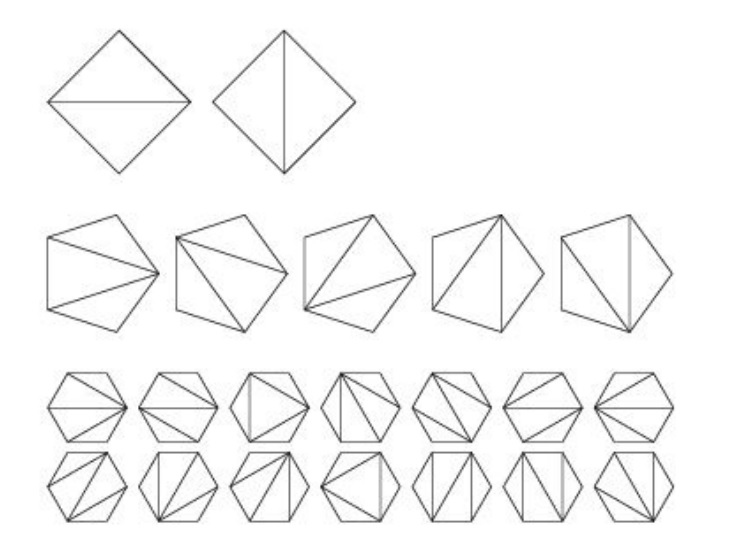
\includegraphics[width=\linewidth]{figures/polygons.jpg}
  \caption{Triangulations for 4, 5, and 6 sided polygons.}
  \label{fig:triangs1}
\end{figure}\\
The rules for triangulation are only such that there are no crossings between the lines. Note: a triangulation of an n-gon uses n-3 line segments and results in n-2 interior triangles.\\
As we can see from Figure 1, the answer to our original question is 14, but let us instead try to come up with a general formula for $T_n = $ number of ways to $\triangle$ a n-gon.\\
\\
Note: The following graphics will be done in Microsoft Paint. I'm sorry in advance.\\


\begin{theorem}
	$$T_n = \sum_{k=2}^{n-1}T_{n-(k-1)}\cdot T_{k-1}$$
\end{theorem}
\begin{proof}
	\textcolor{red}{WARNING: THIS WAS THE PROOF THAT WAS SHOWN IN CLASS THAT HAD AN ERROR IN IT. I still think it is worth to look it over and see why it doesn't work. Just to clarify, although this proof does give the correct recursion, it is not correct. To my knowledge, it is nothing short of a miracle that this method accidentally over-counts and under-counts solutions in such a way to produce a correct recursion.}
	\begin{figure}
        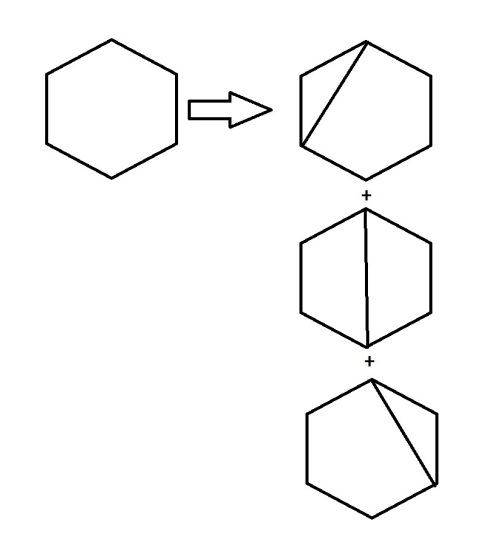
\includegraphics[width=\linewidth]{figures/T6Hexagons.jpg}
        \caption{(Incorrect) recursion for a hexagon.}
        \label{fig:hex1}
    \end{figure}\\
    This hexagon could be broken up into 3 different shapes like this, which would result in $T_6 = T_3\cdot T_5 + T_4\cdot T_4 + T_5\cdot T_3$. This obviously satisfies our original theorem, and all n-gons could be split like this, but this does over-count, because it does not account for when splitting up the remaining polygons you end up with the same triangulation. That is the reason why this proof does not work well for formulating the Catalan numbers.
\end{proof}
\begin{proof}
    Instead of splitting the polygon with a line, which allows for over-counting, if it is instead split with a triangle, we are guaranteed that each solution found is unique, and from looking at the diagram below, we see that the sum of each of these will give us the correct number.
    \begin{figure}
        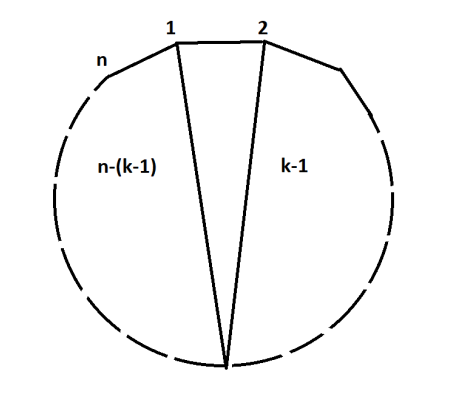
\includegraphics[width=\linewidth]{figures/correctHexagon.png}
        \caption{Correct recursion for a hexagon.}
        \label{fig:hex2}
    \end{figure}\\
\end{proof}

\label{11-0226-1}
\subsection{Triangulating Polygons (Review of Catalan Number Proof)}
\begin{proof}
The number of ways to triangulate a hexagon, $T_6$, can be found by recursion through dividing the interior of the hexagon with a triangle. After picking the triangle in one of 4 ways, the number of ways to triangulate the remaining area is either $T_5T_2$ or $T_4T_3$, depending on the triangle picked. This means we can say $T_6=T_5T_2+T_4T_3+T_3T_4+T_2T_5$. We can shift the indices here to get the recursive definition of Catalan numbers using the following:
\newline
$T_{n+1}=T_2T_n+T_3T_{n-1}+...T_nT_2$
\newline
$T_{n+1}=\sum_{j=2}^{n} {T_jT_{n+2-j}}$
\newline
Let $T_{n+1}=C_n$
\newline
$T_{n+2}=\sum_{j=2}^{n+1} {T_jT_{n+3-j}}$
\newline
$C_n=\sum_{j=2}^{n+1} {C_{j-2}C_{n+1-j}}$
\newline
$C_{n+1}=\sum_{j=2}^{n+1} {C_{j-2}C_{n+2-j}}$
\newline
%%IRIS UWU I'M KINDA UNSURE ABT THIS SO CHECK PLS
$C_{n+1}=\sum_{j=1}^{n} {C_{j}C_{n-j}}$
This is the recursive definition of Catalan numbers, so we can conclude that there are $C_n$ ways to triangulate an n+2-gon. 
\end{proof}

\subsection{Paths (Catalan Numbers II)}
Q: How many paths are there between the points (0, 0) and (2n, 0), only moving with steps of either northeast (up one right one) or southeast (down one right one).\\ (Note: This is analogous to the question of paths between (0, 0) and (n, n) with only vertical and horizontal steps except the algebra works better in this one. However, the pictures I can find are using this interpretation of the problem, so unless we want more Microsoft Paint pictures, these will do. If at any point you get confused between what we did in class and the pictures I'm showing, turn your head $45^\circ$ to the left and it will make sense again.)\\
A: $\binom{2n} n$. 
\begin{proof}
    There are 2n moves, n of them must be up, n must be down, so choose which n will go southeast and we are done.\\
\end{proof}

\begin{figure}
    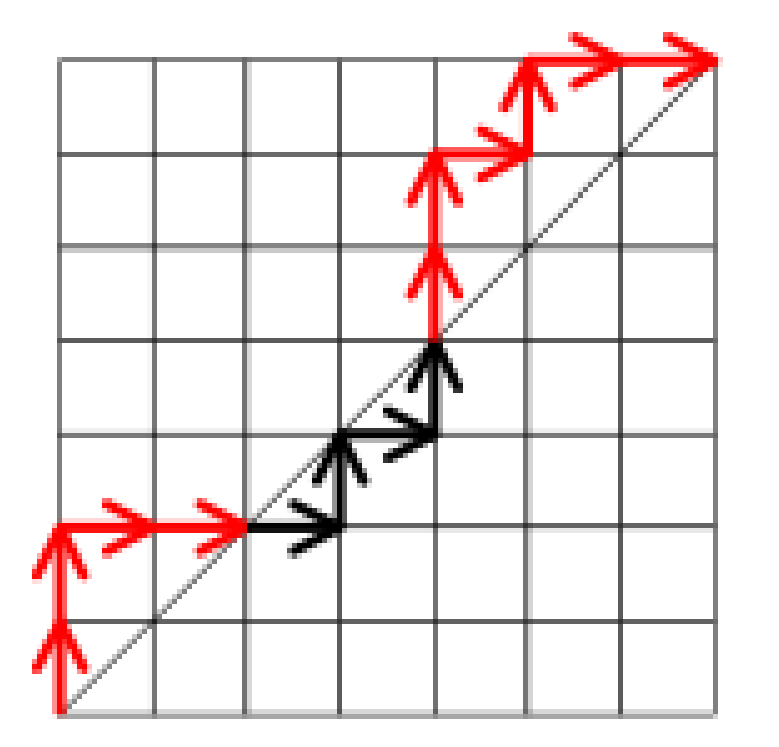
\includegraphics[width=\linewidth]{figures/Catalan_number_exceedance_example.png}
    \caption{An example of a path.}
     \label{fig:hex3}
\end{figure}

Now we want to count all of the paths that do not cross the x-axis, as the one in Figure 4 does. I'm going to have to use paint for this as I cannot find pictures. Sorry again. 

In order to do this, we first notice that all bad paths (ones that cross the x axis), touch the line y = -1 at least once. To count them, we will reflect everything BEFORE the first y = -1 touch along the line y = -1, and leave everything after it the same. (This is why we do it this way instead of diagonally because the reflection is much easier to visualize). This creates a mapping of all bad paths to something else. This is a one to one mapping, every bad path has a reflection, and every reflection has only 1 bad path associated with it. Now, by counting the reflections we also count bad paths. Since the bad paths start at y = -2, and need to reach (2n, 0), we have to choose n+1 up moves (note that this is because this will also result in one less down move, leaving us two above our initial position). \\So bad paths = $\binom{2n}{n-1}$
\\
\\
This gives our total amount of good paths to be the following $$P = \binom{2n}{n} - \binom{2n}{n+1}$$ $$\frac{(2n)!}{n!\cdot n!}-\frac{(2n)!}{(n-1)!(n+1)!} = \frac{(2n)!}{n!\cdot n!} \cdot(1-\frac{n}{n+1})$$
$$= \frac{1}{n+1}\binom{2n} n$$
Which is the Catalan numbers (note how by splitting up the original path problem into two smaller ones, we can also achieve the recursion relation for the Catalan numbers, like we did with the hexagons).

\begin{figure}
    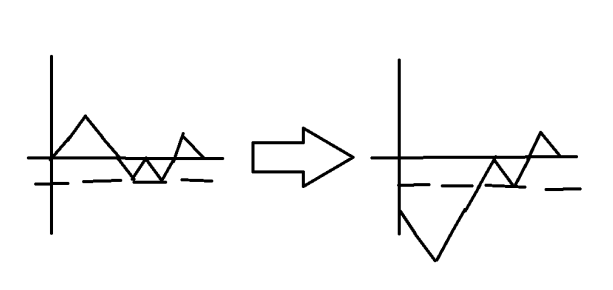
\includegraphics[width=\linewidth]{figures/CatalanAgain.png}
    \caption{The transformation applied to all bad paths}
     \label{fig:hex4}
\end{figure}
% \end{document}
 

\label{09-0221}
%%%%%%% Lecture Notes Style for Concrete Mathematics %%%%%%%%%%%%%
%%%%%%% Taught by Patrick White, TJHSST %%%%%%%%%%%%%%%%%%%%%%%%%%

% \documentclass[11pt,twosided]{article}
% %%%%%%%%%%%%%%%%%%%%%%%%%%%%%%%%%%%%%%%%%%%%%%%%%%%%%%%
%%%% HEADER FILE for CONCRETE MATH LECTURE NOTES %%%%%%
%%%%%%%%%%%%%%%%%%%%%%%%%%%%%%%%%%%%%%%%%%%%%%%%%%%%%%%

%%%%%%%%%%%%%%%%%%%%%%%%%%%%%%%%%%%%%%%%%%%%%%%%%%%%%%%%%%%%%%%%%%%
%% This file is included at the top of every lecture notes file %%%
%% It should ONLY be changed by the instructor %%
%%%%%%%%%%%%%%%%%%%%%%%%%%%%%%%%%%%%%%%%%%%%%%%%%%%%%%%%%%%%%%%%%%%

%%%%%%%%%%%%%%%%%%%%%% package inclusions %%%%%%%%%%%%%%%%%%%%
%\usepackage[
%top=2cm,
%bottom=2cm,
%left=3cm,
%right=2cm,
%headheight=17pt, % as per the warning by fancyhdr
%includehead,includefoot,
%heightrounded, % to avoid spurious underfull messages
%]{geometry} 


\usepackage{amsmath,amssymb,amsfonts}
\usepackage{longtable}
\usepackage{mathtools}
\usepackage{amsthm}
\usepackage{enumerate}
\usepackage{fancyhdr}
\pagestyle{fancy}


%%%%%%%%%%%%%%% theorem style definitions %%%%%%%%%%%%%%%%%%%%%%
\newtheorem{theorem}{Theorem}[section]
%\newtheorem{corollary}{Corollary}[theorem]
%\newtheorem{lemma}[theorem]{Lemma}
\newtheorem*{remark}{Remark}
%\newtheorem{example}{Example}[section]
\newtheorem*{definition}{Definition}


%%%%%%%%%%%%%%%% custom function definitions %%%%%%%%%%%%%%%%%%%%%%%%%
%%%%%%%%%%% as class progresses, this section may be enhanced %%%%%%%%

\def\multiset#1#2{\ensuremath{\left(\kern-.3em\left(\genfrac{}{}{0pt}{}{#1}{#2}\right)
		\kern-.3em\right)}} %%% multiset notation
\newcommand\rf[2]{{#1}^{\overline{#2}}} %%%% rising factorial \rf{x}{m}
\newcommand\ff[2]{{#1}^{\underline{#2}}} %%%%% falling factorial \ff{x}{m}
\newcommand{\Perm}[2]{{}^{#1}\!P_{#2}} % permutation
\newcommand{\half}{\ensuremath{\frac{1}{2}}}
\newcommand{\braces}[1]{\left\{#1\right\}}
\newcommand{\set}[1]{\braces{#1}}
\newcommand{\snb}[2]{\ensuremath{\left(\kern-.3em\left(\genfrac{}{}{0pt}{}{#1}{#2}\right)\kern-.3em\right)}}
\newcommand{\fallingfactorial}[1]{^{\underline{#1}}}
\newcommand{\fallfac}[2]{{#1}^{\underline{#2}}}
\newcommand{\stirlingone}[2]{\genfrac[]{0pt}{1}{#1}{#2}}
\newcommand{\stiri}[2]{\stirlingone{#1}{#2}}
\newcommand{\dstirlingone}[2]{\genfrac[]{0pt}{0}{#1}{#2}}
\newcommand{\dstiri}[2]{\dstirlingone{#1}{#2}}
\newcommand{\stirlingtwo}[2]{\genfrac\{\}{0pt}{1}{#1}{#2}}
\newcommand{\stirii}[2]{\stirlingtwo{#1}{#2}}
\newcommand{\dstirlingtwo}[2]{\genfrac\{\}{0pt}{0}{#1}{#2}}
\newcommand{\dstirii}[2]{\dstirlingtwo{#1}{#2}}
\newcommand{\ol}[1]{\overline{#1}}
%%%%%%%
% book stuff
%%%%%%%%%

\usepackage[twoside,outer=1.5in,inner=2in,bottom=1.5in,top=1.5in,marginpar=2in]{geometry} 
\usepackage{scrextend}
\usepackage{palatino}
\usepackage{multicol}
\usepackage{float}
\usepackage[hidelinks]{hyperref}
\usepackage[nameinlink, capitalise, noabbrev]{cleveref}
%\usepackage{background}
\usepackage{graphicx}
\usepackage{listliketab}

\usepackage{lipsum}
\usepackage{caption}
\usepackage{marginnote}

\reversemarginpar


\usepackage[dvipsnames]{xcolor}
\usepackage{amsthm}
\usepackage{shadethm}

\setlength{\parindent}{0pt}

\newcommand*\Note{%
	\marginnote[\textcolor{blue}{\raggedright{\LARGE ?}\ Note }]{}%
}
\newcommand*\Warn{%
	\marginnote[\textcolor{red}{\raggedright{\LARGE !}\ Warning }]{}%
}
\reversemarginpar

\newcommand{\N}{\mathbb{N}}
\newcommand{\Z}{\mathbb{Z}}
\newcommand{\I}{\mathbb{I}}
\newcommand{\R}{\mathbb{R}}
\newcommand{\Q}{\mathbb{Q}}
\renewcommand{\qed}{\hfill$\blacksquare$}
\let\newproof\proof
\renewenvironment{proof}{\begin{addmargin}[1em]{0em}\begin{newproof}}{\end{newproof}\end{addmargin}\qed}
% \newcommand{\expl}[1]{\text{\hfill[#1]}$}


\newenvironment{lemma}[2][Lemma]{\begin{trivlist}
		\item[\hskip \labelsep {\bfseries #1}\hskip \labelsep {\bfseries #2.}]}{\end{trivlist}}
\newenvironment{problem}[2][Problem]{\begin{trivlist}
		\item[\hskip \labelsep {\bfseries #1}\hskip \labelsep {\bfseries #2.}]}{\end{trivlist}}
\newenvironment{example}[2][Example]{\begin{trivlist}
		\item[\hskip \labelsep {\bfseries #1}\hskip \labelsep{\bfseries #2.}]}{\end{trivlist}}
\newenvironment{solution}{{\noindent \bfseries Solution\hskip 2ex}}{\qed}
\newenvironment{exercise}[2][Exercise]{\begin{trivlist}
		\item[\hskip \labelsep {\bfseries #1}\hskip \labelsep {\bfseries #2.}]}{\end{trivlist}}
\newenvironment{reflection}[2][Reflection]{\begin{trivlist}
		\item[\hskip \labelsep {\bfseries #1}\hskip \labelsep {\bfseries #2.}]}{\end{trivlist}}
\newenvironment{proposition}[2][Proposition]{\begin{trivlist}
		\item[\hskip \labelsep {\bfseries #1}\hskip \labelsep {\bfseries #2.}]}{\end{trivlist}}
\newenvironment{corollary}[2][Corollary]{\begin{trivlist}
		\item[\hskip \labelsep {\bfseries #1}\hskip \labelsep {\bfseries #2.}]}{\end{trivlist}}

%%%% add package inclusions here, if any

%%%%% Define your custom functions and macros here, if any

%%%%%%%%%%%%%%%%%%%% Define the variables below %%%%%%%%%%%%%%%%%%%%%%%%%%%%%%
% \def\titlestring{Properties of n!}
% \def\scribestring{Varun Gannavarapu}
% \def\datestring{21 February 2019}


%%%%%%%%%%%%%%%%%%% Page Headers -- Do Not Change %%%%%%%%%%%%%%%%%%%%%%%%%%%
% \lhead{\titlestring}
% \rhead{Page \thepage}
% \cfoot{Concrete Math -- White -- TJHSST}
% \renewcommand{\headrulewidth}{0.4pt}
% \renewcommand{\footrulewidth}{0.4pt}

%%%%%%%%%%%%%%%%% Begin the document %%%%%%%%%%%%%%%%%%%%%%%%%
% \begin{document}
% \thispagestyle{plain}  %% no headers on this page

% %%%% Do not change these lines %%%%%
% \noindent
% {\LARGE \textbf{\titlestring}}\\\\
% %
% {\Large Scribe: \scribestring}\\ \\
% {\textbf{Date}: \datestring}


%%%%%%%%%%%%%%%%%%%%%%%%%% YOUR CONTENT GOES HERE %%%%%%%%%%%%%%%%%%%%%%%%%%
\noindent

\section{Interlude: Stirling's Approximation}
We intend to examine different ways that we may approximate the value of $n!$. The first of these methods is Stirling's Approximation.\\
\begin{theorem}
    (Stirling's Approximation) $\lim_{n\to\infty} \frac{n!}{(\frac{n}{e})^n * \sqrt{2\pi n}} = 1$
\end{theorem}
This is the formal definition of Stirling's Approximation. The actual approximation that we are observing, would be the denominator of this fraction. Stirling's thinking behind this, is that as $n$ increases in size, the ratio should eventually become equal to $1$.\\
We won't however, be proving the formal definition of Stirling's Approximation. Instead, we want to find some sort of upper and lower bound for the value of $n!$. To do this, we will first create an informal definition for $n!$.\\
\\
Informally speaking, $n! \sim \frac n e ^n * \sqrt{2\pi n}$\\
We intend to prove that $n! = \frac n e ^n * \delta \sqrt{n}$, where $\delta \cong \sqrt{2\pi}$\\
\\
To do this proof, we also want to make note of an important summation remark:
\begin{remark}
    $log(n!) = \sum_{i=1}^{n} {log(i)}$\\
\end{remark}

\begin{proof}
To do the actual proof, we will consider the function $y=ln(x)$. From here we intend to make two Riemann-style approximations for the integral $\int_{i}^{n}{ln(x)dx}$. For our proof, both approximations will be trapezoidal approximations. \\

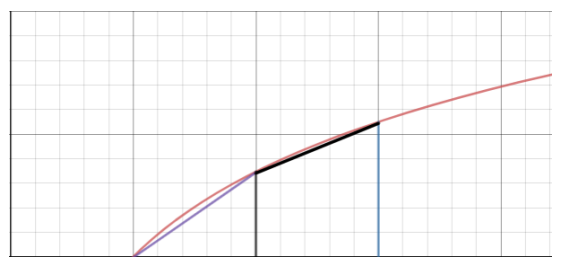
\includegraphics[width=20\baselineskip]{figures/trapezoidal_under.png}\\
Approach one is two use a trapezoid whose bases are at the integers themselves.\\

Area of the trapezoids is $\frac{1}{2}\sum_{i=1}^{n-1}{[ln(i)+ln(i+1)]}$\\
$=\frac{1}{2}ln(1)+\sum_{i=2}^{n-1}{[ln(i)+ln(i+1)]}+\frac{1}{2}ln(n)$\\
$=ln(n!)-\frac{1}{2}ln(n)$\\

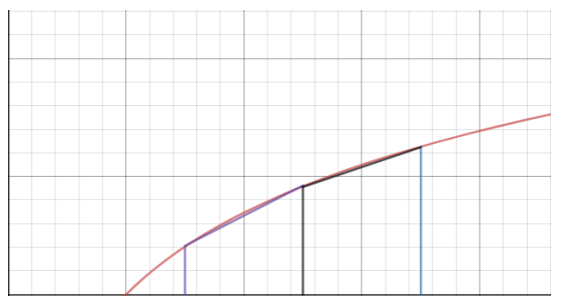
\includegraphics[width=20\baselineskip]{figures/trapezoidal_over.png}\\
Approach two is two use a trapezoid whose bases are at the midpoints between integers. Notice that we don't care about the area before $x=\frac{1}{2}$ in our calculations.\\ 

Area = $ln(2)+ln(3)+ln(4)\dots+ln(n-1)+\frac{1}{2}ln(n)$, which comes out to be the same as above.  Notice that this is an overestimate however, and the previous approach was an underestimate.\\
$\therefore \int_{\frac{3}{2}}^{n}{ln(x)}dx + \frac{1}{2}ln(n) < ln(n!) < \int_{1}^{n}{ln(x)}dx + \frac{1}{2}ln(n)$\\

Given $\int{ln(x)}dx = xln(x) - x + C$\\

We get:\\
$(nln(n)-n)-(\frac{3}{2}ln(\frac{3}{2}) - \frac{3}{2}) + \frac{1}{2}ln(n) < ln(n!) < (nln(n) - n) - (ln(1) - 1) + \frac{1}{2}ln(n)$\\
$=(n+\frac{1}{2})ln(n)-n-\frac{3}{2}(ln(\frac{3}{2}) - 1) < ln(n!) < (n+\frac{1}{2})ln(n) - n + 1$\\

At this point, we have a range of error for $ln(n!)$.\\

We can define $ln(n!) = [(n+\frac{1}{2})ln(n) - n] + \delta_n$, where $\frac{3}{2}(1-ln(\frac{3}{2})) < \delta_n < 1 \longrightarrow 0.891802 < \delta_n < 1$\\

Since $ln(n!) = (n+\frac{1}{2})ln(n) - n + \delta_n$,\\
$e^{ln(n!)} = e^{nln(n)}e^{\frac{1}{2}ln(n)}e^{-n}e^{\delta_n}$\\
$n! = n^n \sqrt(n) e^{-n}e^{\delta_n}$\\
$=(\frac{n}{e})^n \sqrt(n) * e^{\delta_n}$, where $e^{\delta_n} \in [2.439, 2.718]$. The value for $\sqrt{2 \pi n} = 2.506$, which falls within our expected range of values.

\end{proof}

Now that we have an approximation for $n!$, we can look to write an expression that will give us the $n^{th}$ Catalan number. The $n^{th}$ Catalan number is given by the expression $\binom {2n} n*\frac{1}{n+1}$\\
$\binom{2n}n*\frac{1}{n+1} = \frac{(2n)!}{n!n!} = \frac{(2n)!}{[(\frac{n}{e})^n * \sqrt{2\pi n}]^2}$\\
$= \frac{\frac{2n}{e}^{2n}}{\frac{n}{e}^{2n}} * \frac{\sqrt{4\pi n}}{2\pi n * (n+1)} = \frac{2^{2n}*\sqrt{\pi n}}{\pi n(n+1)} = \frac{4^n}{\sqrt{\pi n}(n+1)}$

\subsection{Gamma Function}
Gamma functions are an extension of factorials, such that the arguments are shifted down by one. In other words, $\Gamma(2) = 1!$, $\Gamma(3) = 2!$, etc. We intend to prove that $\Gamma(n+1) = n!$. To do this, we first begin by defining our gamma function.\\
\begin{definition}
    $\Gamma(z+1)=\int_{0}^{\infty} {x^{z}e^{-x}}$
\end{definition}
Now that we have defined our gamma function, we will attempt to prove that $\Gamma(n+1) = n!$.\\
\begin{proof}
First, we will integrate this function by parts:
\begin{multicols}{2}
\begin{itemize}
    \item $u = x^7$, $du = zx^{z-1}$
    \item $v = -e^{-x}$, $dv=e^{-x}$
\end{itemize}
\end{multicols}
$\therefore \int_{0}^{\infty}{x^{z}e^{-x}dx} = [x^{z}(-e^{-x})]_{0}^{\infty} + \int_{0}^{\infty}{zx^{z-1}e^{-x}dx}$\\

Notice how when we evaluate the expression $\int_{0}^{\infty}{x^{z}e^{-x}dx} = [x^{z}(-e^{-x})]_{0}^{\infty}$, $x^{z}$ becomes $0$ when evaluated at $x=0$, and $(-e^{-x})$ becomes zero when evaluated at $x=\infty$, meaning that this expression evaluates to just $0$. \\

Therefore, we are left with just $\int_{0}^{\infty}{zx^{z-1}e^{-x}dx}$. We can redefine this as $z\int_{0}^{\infty}{x^{z-1}e^{-x}dx} = z\Gamma(z)$.\\

At this point, we have something that is similar to a factorial, but we can't consider our proof complete until we establish some base cases. We can begin by testing with $z=1$. $\Gamma(1) = \int_{0}^{\infty}{x^{0}e^{-x}}dx = \int_{0}^{\infty}{e^{-x}}dx = 1$\\
$\therefore \Gamma(1) = 1$\\
$\Gamma(2) = 1 * \Gamma(1) = 1$\\
$\Gamma(3) = 2 * \Gamma(2) = 3$\\
$\Gamma(4) = 3 * \Gamma(3) = 6$\\
$\therefore \Gamma(n+1) = n!$
\end{proof}
As we intended, we have now found a function that is similar to a factorial, withe the arguments shifted by one. However, we also want to observe how fractional factorials work. In our case, we'll observe $\Gamma(\frac{1}{2})$. 
\begin{proof}
$\Gamma(\frac{1}{2})=\int_{0}^{\infty}{x^{\frac{-1}{2}}e^{-x}}dx = \int_{0}^{\infty}{\frac{e^{-x}}{\sqrt{x}}}$\\
Let $u=\sqrt{x}$, $u^2=x$, and $du*2u=dx$\\
Substituting $u$ into the equation, we get $\Gamma(\frac{1}{2})=2\int_{0}^{\infty}{e^{-u^2}}du$\\
Now suppose we define a variables $v$ and $K$, such that\\
$K=\int_{0}^{\infty}{e^{-u^2}}du = \int_{0}^{\infty}{e^{-v^2}}dv$\\
$K^2=\int_{0}^{\infty}{e^{-u^2}}du \int_{0}^{\infty}{e^{-v^2}}dv$\\
$=\int_{0}^{\infty}\int_{0}^{\infty}{e^{-u^2}e^{-v^2}}dudv = \int_{0}^{\infty}\int_{0}^{\infty}{e^{-(u^2+v^2)}}dudv$\\
In Cartesian coordinates, this integral would be difficult to solve. However, we can convert to polar coordinates to solve this equation. Notice that because we are only using positive integers, $\theta$ is bounded within the first quadrant\\
$K^2=\int_{0}^{\frac{\pi}{2}}\int_{0}^{\infty}{e^{-r^2}*r}drd\theta = \frac{\pi}{2}\int_{0}^{\infty}{e^{-r^2}*r}dr$\\
$=\frac{\pi}{2}*(\frac{-e^{-r^2}}{2})_{0}^{\infty} = \frac{\pi}{2}(\frac{1}{2} - 0) = \frac{\pi}{4}$\\
$\therefore K = \frac{\sqrt{\pi}}{2}$\\
$\therefore \Gamma(\frac{1}{2}) = 2K = 2\frac{\sqrt{\pi}}{2} = \sqrt{\pi}$
\end{proof}
% \end{document}


\label{11-0226-2}
%%%%%%% Lecture Notes Style for Concrete Mathematics %%%%%%%%%%%%%
%%%%%%% Taught by Patrick White, TJHSST %%%%%%%%%%%%%%%%%%%%%%%%%%

% \documentclass[11pt,twosided]{article}
% %%%%%%%%%%%%%%%%%%%%%%%%%%%%%%%%%%%%%%%%%%%%%%%%%%%%%%%
%%%% HEADER FILE for CONCRETE MATH LECTURE NOTES %%%%%%
%%%%%%%%%%%%%%%%%%%%%%%%%%%%%%%%%%%%%%%%%%%%%%%%%%%%%%%

%%%%%%%%%%%%%%%%%%%%%%%%%%%%%%%%%%%%%%%%%%%%%%%%%%%%%%%%%%%%%%%%%%%
%% This file is included at the top of every lecture notes file %%%
%% It should ONLY be changed by the instructor %%
%%%%%%%%%%%%%%%%%%%%%%%%%%%%%%%%%%%%%%%%%%%%%%%%%%%%%%%%%%%%%%%%%%%

%%%%%%%%%%%%%%%%%%%%%% package inclusions %%%%%%%%%%%%%%%%%%%%
%\usepackage[
%top=2cm,
%bottom=2cm,
%left=3cm,
%right=2cm,
%headheight=17pt, % as per the warning by fancyhdr
%includehead,includefoot,
%heightrounded, % to avoid spurious underfull messages
%]{geometry} 


\usepackage{amsmath,amssymb,amsfonts}
\usepackage{longtable}
\usepackage{mathtools}
\usepackage{amsthm}
\usepackage{enumerate}
\usepackage{fancyhdr}
\pagestyle{fancy}


%%%%%%%%%%%%%%% theorem style definitions %%%%%%%%%%%%%%%%%%%%%%
\newtheorem{theorem}{Theorem}[section]
%\newtheorem{corollary}{Corollary}[theorem]
%\newtheorem{lemma}[theorem]{Lemma}
\newtheorem*{remark}{Remark}
%\newtheorem{example}{Example}[section]
\newtheorem*{definition}{Definition}


%%%%%%%%%%%%%%%% custom function definitions %%%%%%%%%%%%%%%%%%%%%%%%%
%%%%%%%%%%% as class progresses, this section may be enhanced %%%%%%%%

\def\multiset#1#2{\ensuremath{\left(\kern-.3em\left(\genfrac{}{}{0pt}{}{#1}{#2}\right)
		\kern-.3em\right)}} %%% multiset notation
\newcommand\rf[2]{{#1}^{\overline{#2}}} %%%% rising factorial \rf{x}{m}
\newcommand\ff[2]{{#1}^{\underline{#2}}} %%%%% falling factorial \ff{x}{m}
\newcommand{\Perm}[2]{{}^{#1}\!P_{#2}} % permutation
\newcommand{\half}{\ensuremath{\frac{1}{2}}}
\newcommand{\braces}[1]{\left\{#1\right\}}
\newcommand{\set}[1]{\braces{#1}}
\newcommand{\snb}[2]{\ensuremath{\left(\kern-.3em\left(\genfrac{}{}{0pt}{}{#1}{#2}\right)\kern-.3em\right)}}
\newcommand{\fallingfactorial}[1]{^{\underline{#1}}}
\newcommand{\fallfac}[2]{{#1}^{\underline{#2}}}
\newcommand{\stirlingone}[2]{\genfrac[]{0pt}{1}{#1}{#2}}
\newcommand{\stiri}[2]{\stirlingone{#1}{#2}}
\newcommand{\dstirlingone}[2]{\genfrac[]{0pt}{0}{#1}{#2}}
\newcommand{\dstiri}[2]{\dstirlingone{#1}{#2}}
\newcommand{\stirlingtwo}[2]{\genfrac\{\}{0pt}{1}{#1}{#2}}
\newcommand{\stirii}[2]{\stirlingtwo{#1}{#2}}
\newcommand{\dstirlingtwo}[2]{\genfrac\{\}{0pt}{0}{#1}{#2}}
\newcommand{\dstirii}[2]{\dstirlingtwo{#1}{#2}}
\newcommand{\ol}[1]{\overline{#1}}
%%%%%%%
% book stuff
%%%%%%%%%

\usepackage[twoside,outer=1.5in,inner=2in,bottom=1.5in,top=1.5in,marginpar=2in]{geometry} 
\usepackage{scrextend}
\usepackage{palatino}
\usepackage{multicol}
\usepackage{float}
\usepackage[hidelinks]{hyperref}
\usepackage[nameinlink, capitalise, noabbrev]{cleveref}
%\usepackage{background}
\usepackage{graphicx}
\usepackage{listliketab}

\usepackage{lipsum}
\usepackage{caption}
\usepackage{marginnote}

\reversemarginpar


\usepackage[dvipsnames]{xcolor}
\usepackage{amsthm}
\usepackage{shadethm}

\setlength{\parindent}{0pt}

\newcommand*\Note{%
	\marginnote[\textcolor{blue}{\raggedright{\LARGE ?}\ Note }]{}%
}
\newcommand*\Warn{%
	\marginnote[\textcolor{red}{\raggedright{\LARGE !}\ Warning }]{}%
}
\reversemarginpar

\newcommand{\N}{\mathbb{N}}
\newcommand{\Z}{\mathbb{Z}}
\newcommand{\I}{\mathbb{I}}
\newcommand{\R}{\mathbb{R}}
\newcommand{\Q}{\mathbb{Q}}
\renewcommand{\qed}{\hfill$\blacksquare$}
\let\newproof\proof
\renewenvironment{proof}{\begin{addmargin}[1em]{0em}\begin{newproof}}{\end{newproof}\end{addmargin}\qed}
% \newcommand{\expl}[1]{\text{\hfill[#1]}$}


\newenvironment{lemma}[2][Lemma]{\begin{trivlist}
		\item[\hskip \labelsep {\bfseries #1}\hskip \labelsep {\bfseries #2.}]}{\end{trivlist}}
\newenvironment{problem}[2][Problem]{\begin{trivlist}
		\item[\hskip \labelsep {\bfseries #1}\hskip \labelsep {\bfseries #2.}]}{\end{trivlist}}
\newenvironment{example}[2][Example]{\begin{trivlist}
		\item[\hskip \labelsep {\bfseries #1}\hskip \labelsep{\bfseries #2.}]}{\end{trivlist}}
\newenvironment{solution}{{\noindent \bfseries Solution\hskip 2ex}}{\qed}
\newenvironment{exercise}[2][Exercise]{\begin{trivlist}
		\item[\hskip \labelsep {\bfseries #1}\hskip \labelsep {\bfseries #2.}]}{\end{trivlist}}
\newenvironment{reflection}[2][Reflection]{\begin{trivlist}
		\item[\hskip \labelsep {\bfseries #1}\hskip \labelsep {\bfseries #2.}]}{\end{trivlist}}
\newenvironment{proposition}[2][Proposition]{\begin{trivlist}
		\item[\hskip \labelsep {\bfseries #1}\hskip \labelsep {\bfseries #2.}]}{\end{trivlist}}
\newenvironment{corollary}[2][Corollary]{\begin{trivlist}
		\item[\hskip \labelsep {\bfseries #1}\hskip \labelsep {\bfseries #2.}]}{\end{trivlist}}

% %%%% add package inclusions here, if any

% %%%%% Define your custom functions and macros here, if any

% %%%%%%%%%%%%%%%%%%%% Define the variables below %%%%%%%%%%%%%%%%%%%%%%%%%%%%%%
% \def\titlestring{02/26/19 Lecture}
% \def\scribestring{Sabrina Cai and Iris Wu}
% \def\datestring{2/26/19}


% %%%%%%%%%%%%%%%%%%% Page Headers -- Do Not Change %%%%%%%%%%%%%%%%%%%%%%%%%%%
% \lhead{\titlestring}
% \rhead{Page \thepage}
% \cfoot{Concrete Math -- White -- TJHSST}
% \renewcommand{\headrulewidth}{0.4pt}
% \renewcommand{\footrulewidth}{0.4pt}

% %%%%%%%%%%%%%%%%% Begin the document %%%%%%%%%%%%%%%%%%%%%%%%%
% \begin{document}
% \thispagestyle{plain}  %% no headers on this page

% %%%% Do not change these lines %%%%%
% \noindent
% {\LARGE \textbf{\titlestring}}\\\\
% %
% {\Large \scribestring}\\ \\
% {\textbf{Date}: \datestring}


%%%%%%%%%%%%%%%%%%%%%%%%%% YOUR CONTENT GOES HERE %%%%%%%%%%%%%%%%%%%%%%%%%%
\noindent


\section{Problems and Examples}

\label{21-0321-1}
\subsection{Remark: Unlabeled Probability}

\begin{problem}
1 You throw two marbles into two buckets. Find the probability that they both land in the same bucket: 

\begin{itemize}
    \item Unlabeled into unlabeled:  1/2 (2 scenarios: marbles in separate buckets or together)
    \item Labeled into unlabeled: 1/2 (2 scenarios: marbles in separate buckets or together)
    \item Labeled into labeled: 1/2 (4 scenarios - 2 of which include both marbles in the same bucket)
    
    \item Unlabeled into labeled: 
    
    Let's label buckets A and B. You have two indistinguishable marbles, and so there are three scenarios: marbles are in separate buckets, both marbles are in A, and both marbles in B. Therefore, you may incorrectly conclude that the probability is 2/3, when in reality it remains 1/2. The probability of marbles being in separate buckets is twice the odds that both marbles are in A. 
    \newline \newline
    This is because \textbf{probability problems are ALWAYS labeled.}
    \newline \newline
    If you label the marbles 1 and 2, there are two ways for the marbles to be in separate buckets, each as probable as any of the other scenarios: 1-A and 2-B or 1-B and 2-A. 
    
    When you are asked for the probability, always treat both the balls and urns, or marbles and buckets, as labeled into labeled. 

\end{itemize}

\end{problem}

\subsection{Homework Problems (Problem Set 2)}
%%% Question 1

\begin{problem}{1}
    In how many ways may we write n as a sum of an ordered list of k positive numbers? Such a list is called a composition of n into k parts.
\end{problem}
\begin{solution}
    We can split n into n identical 1's. Then the problem becomes about dividing identical objects into k distinguishable piles with at least one in each pile to form ordered pairs of numbers which sum to n. That makes this stars and bars where we have k-1 bars (to divide the set into k-1 groups) and n-1 possible spaces (we want at least one 1 in each group). There are $\binom{n-1}{k-1}$ ways to do this.
\end{solution}

%%% Question 2

\begin{problem} 2
    What is the total number of compositions of n (into any number of parts).
\end{problem}
\begin{solution}
    In this question, we have n-1 spaces between each 1 that we can make a "bar" that creates a new group. We have two groups that n-1 things can fall in, so our total number of ways to do that is \(2^{n-1}\). Alternatively, we could recognize that the total number of ways to do this is the sum of our answer from question one where k goes from 1 to n-1 (\(\sum^{n-1}_{k=1}\binom{n-1}{k}\)) matches the form of the sum in the binomial theorem (\((a+b)^{j} = \sum^{j}_{k=0}\binom{j}{k}a^{j-k}b^{k}\)). In this case, a and b would both be 1 and j would be n-1, which would give us \(2^{n-1}\).
\end{solution}

%%% Question 3

\begin{problem} 3
    A Grey Code is an ordering of n-digit binary strings such that each string differs from the previous in precisely one digit.
\end{problem}



%%% Question 3.1
\begin{problem}{3.1}
    {Write one Grey Code for n=4.}
\end{problem}
1111, 1110, 1100, 1000, 0000, 0001, 0011, 0111, 0101, 1101, 1001, 1011, 1010, 0010, 0110, 0100.

%%% Question 3.2

\begin{problem}{3.2}{Prove by induction that Grey Codes exist for all $n \geq{4}$.}\end{problem}
Let n=4 be the base case. Starting with a Grey Code for n=4, to create one for n=5, we can duplicate all the numbers in the Grey Code while keeping the same order and alternate between adding 1's and 0's in the front using the following pattern: 1, 0, 0, 1, 1, 0... This maintains the one-digit difference while listing all the 5-digit binary numbers (because each number listed is unique, since the list of 4-digit numbers was unique and either 0 or 1 is added only once to each number, and there are twice as many numbers in the list, just like there are twice as many 5 digit binary numbers as 4-digit ones). For example, using the earlier Grey Code, we get (11111, 01111, 01110, 11110...). This procedure can be repeated for 6-digit numbers, 7-digit numbers, and so on.

%%% Question 3.3

\begin{problem}{3.3}{Prove that the number of even-sized subsets of an n-element set equals the number of odd-sized subsets of an n-element set.}
\end{problem}
    The subsets of an n-element set can be mapped one-to-one to the strings in a Grey Code for n=n by having the 0's and 1's indicate whether or not to include each element of the original set. Since each string in a Grey Code differs from the previous string by exactly 1 digit, the strings must alternate between having even and odd numbers of 1's, indicating even or odd sized subsets. Since there are $2^n$ binary strings of length n, there are an even number of strings in each Grey Code, so the alternation between odd and even sized subsets must produce equal numbers of both. 

%%% Question 4

\begin{problem} 4 {A list of parentheses is said to be balanced if there are the same number of left parentheses as right, and as we count from left to right we always find at least as many left parentheses as right parentheses. For example, (((()()))()) is balanced and ((()) and (()()))(() are not. How many balanced lists of n left and n right parentheses are there?}
\end{problem}
    This is equivalent to the problem of counting the number of paths from (0, 0) to (2n, 0) using only northeast (1, 1) and southeast (1, -1) steps without crossing the x-axis. Adding left parentheses translates to moving northeast, and adding right parentheses translates to moving southeast. Their numbers must be equal in the end, and not crossing the x-axis ensures that the number of left parentheses is always at least as many as the number of right parentheses. To count the number of paths, we use complementary counting: there are $\binom{2n}n$ paths altogether, and $\binom{2n}{n+1}$ paths that cross the x-axis (which we can count by reflecting them across the line y=-1 to form paths from (0, -2) to (2n, 0)). This results in \(\frac{\binom{2n}{n}}{n+1}\) acceptable paths and acceptable lists. 

%%% Question 5

\begin{problem} 5 {A tennis club has 4n members. To specify a doubles match, we choose two teams of two people. In how many ways may we arrange the members into doubles matches so that each player is in one doubles match? In how many ways may we do it if we specify in addition who serves first on each team?}
\end{problem}
    We can start by arranging the 4n people into a line, which can be done in (4n)! ways. We can then assign them to courts by taking the first 4 people for the first court, the next 4 for the second, and so on. Since the order of the courts doesn't matter, we must divide by n!. Then, we must account for another overcounting issue: we have 8 different ways to specify the same set of 2 teams for each court. To account for this issue, we must divide by $2^{(3n)}$, since there are n courts. Altogether, this gives us \(\frac{(4n)!}{n! \times 2^{3n}}\) ways.

%%% Question 6

\begin{problem} 6 {A town has n streetlights running along the north side of main street. The poles on which they are mounted need to be painted so that they do not rust. In how many ways may they be painted with red, white, blue, and green if an even number of them are to be painted green?}
\end{problem}
    We can start by picking an even number of the n poles to be green: there are $\binom{n}{2k}$ ways to do this, where k ranges from 0 to ${\lfloor {n/2} \rfloor}$ There are 3 ways to color each of the remaining n-2k poles, meaning $3^{n-2k}$ ways altogether. This means the total number of ways to color these streetlights is $\sum_{k=0}^{\lfloor{n/2} \rfloor} {\binom{n}{2k} * 3^{n-2k}}$. We can get the closed form of this by adding the binomial expansions of $(3+1)^n$ and $(3-1)^n$ and dividing by 2 to get the sum. This gives $2^{2n-1}+2^{n-1}$. 
\newline
Alternatively...
\newline
Preview of formulation 3:
\newline
Let $E_n$=number of ways to color n poles with an even number of greens, and $O_n$=number of ways to color n poles with an odd number of greens, so that $E_n$+$O_n$=the total number of ways to color n poles.$E_{n+1}=3E_n+O_n$: Adding one more pole to a set of n poles such that we end up with an even number of green poles can be done in only one way if there are an odd number of green poles in the first set of n poles (the pole must be green) and can be done in 3 ways if there are an even number of green poles in the first n poles (the pole can be any color but green). 

%%% Question 7

\begin{problem} 7 {We have n identical ping pong balls. In how many ways may we paint them red, white, blue, and green if we use green paint on an even number of them?}
%%IRIS CAN YOU READ OVER THIS AND ALSO PUT IN THE MULTISET THING BC I AM HORRIBLE AT LATEX
\end{problem}
There must be 2k balls painted green, where k ranges from 0 to ${\lfloor n/2 \rfloor}$ in order to ensure that the number of green balls is even. There are 3 ways to color each of the remaining n-2k balls. We can imagine this as a multiset problem, where there are n copies of each of the 3 colors. This means there are \(\sum_{k=0}^{\lfloor n/2 \rfloor} \multiset{3}{n-2k}\) ways to color the balls altogether. 

%%% Question 8

\begin{problem} 8 {A boolean function $ f: {(0, 1)}^n $  $\rightarrow $0, 1 is self-dual if replacing all 0s with 1s and 1s with 0s yields the same function. How many self-dual boolean functions are there as a function of n?}
\end{problem}

We can regard the function's inputs to be in pairs, where switching the 0s and 1s of one member of the pair results in the other member. To ensure that the function is self-dual, both members of a pair must give the same result when inputted into f, meaning that there are $2^n$/2 distinct inputs. Since each input can be mapped to 0 or 1, this means the number of possible functions is $2^{2^{n-1}}$.

%%% Question 9

\begin{problem} 9 {A boolean function $ f: {(0, 1)}^n $  $\rightarrow $0, 1 is symmetric if any permutation applied to the digits in the domain yields the same function. e.g. f(001)=f(010)=f(100). How many symmetric boolean functions are there as a function of n?}
\end{problem}
    Again, we can group the function inputs based on which must give the same output. There will now be n input groups based on how many 1s are in the input, since inputs with the same number of 1s are just permutations of each other. This means there are n+1 distinct inputs which can each be mapped to 0 or 1, so the number of possible functions is $2^{n+1}$.

%%% Question 10

\begin{problem}{10}{Prove $x^n$= $\sum_{k=0}^{n} {S(n, k)x^{\underline{k}}}$.}
\end{problem}
The number of ways to assign n labeled balls to k labeled urns is k!S(n, k) if we want at least one ball in each urn. To assign n balls to k urns out of x potential urns, we must assign at least one ball to k urns and no balls to the other x-k. There are k!S(n, k)*$\binom x k$, or $S(n, k)x^{\underline{k}}$ ways to do this. k ranges from 0 to n, since we wanted at least one of the n balls in each of the urns. Summing all the possible values of k up, we get $\sum_{k=0}^{n} {S(n, k)x^{\underline{k}}}$. This is equivalent to the left side of the equation, which corresponds to assigning n labeled balls to x labeled urns with no restrictions. 

%%% Question 11

    \begin{problem}{11}{Prove that $(1+x)^\alpha$=$\sum_{k=0}^{\infty} {\alpha^{\underline{k}}x^k/k!}$ for any real $ \alpha$.}
\end{problem}
    The Taylor series for 1+x centered around 0 is $(1+x)^\alpha+\alpha*x/1!+\alpha*(\alpha-1)*x^2/2!$...which is equivalent to $\sum_{k=0}^{\infty}{\alpha^{\underline{k}}x^k/k!}$

    \subsection{Equivalence Relations (Bell Numbers)}
A relation on set A is a subset of AxA={(a, a), (a, b)...(b, a)...(d, d)}. An equivalence relation is defined as any relation that is symmetric, reflexive, and transitive. 
\newline
Definitions:
\newline
Reflexive - a relates to a, or must relate to itself (e.g., greater than is not a reflexive relationship because a number cannot be greater than itself).
\newline
Transitive - if a relates to b and b relates to c, then a relates to c (e.g., greater than is symmetric because if a \(>\) b and b \(>\) c, then a \(>\) c).
\newline
Symmetric - if a relates to b, then b relates to a (e.g., greater than is not symmetric because if a \(>\) b, b cannot be greater than a).
\newline
Cayely tables represent relations as a table. An example can be found below:
\begin{center}
\begin{tabular} {c|c c c c}
& A & B & C & D \\
\hline
A & X &  &  &  \\
B & X & X &  &  \\
C &  &  &  &  \\
D &  &  &  & X \\
\end{tabular}
\end{center}
This table says that a relates to a, b relates to a, b relates to b, and d relates to d. As an example, this table isn't reflexive, symmetric, or transitive.
The following revised table makes the relation symmetric.
\begin{center}
\begin{tabular} {c|c c c c}
& A & B & C & D \\
\hline
A & X &  &  &  \\
B & X & X &  &  \\
C &  &  & X &  \\
D &  &  &  & X \\
\end{tabular}
\end{center}
The table still isn't transitive or symmetric, though. The next table is symmetric and reflexive, but not transitive.
\begin{center}
\begin{tabular} {c|c c c c}
& A & B & C & D \\
\hline
A & X & X &  &  \\
B & X & X & X &  \\
C &  & X & X &  \\
D &  &  &  & X \\
\end{tabular}
\end{center}
The following table is all three:
\begin{center}
\begin{tabular} {c|c c c c}
& A & B & C & D \\
\hline
A & X & X & X &  \\
B & X & X & X &  \\
C & X & X & X &  \\
D &  &  &  & X \\
\end{tabular}
\end{center}
How can we count how many possible relations are reflexive; reflexive and symmetric; and reflexive, symmetric, and transitive (given n rows and columns)?
\begin{problem}1{How can we count the number of reflexive relations?}\end{problem}
All reflexive relations must have the diagonal filled in. Without the diagonal, there are \(n^{2} - n\) spaces that can be filled in or left empty. Because each space can go two ways, our final answer is \(2^{n^{2}-n}\).
\begin{problem}2{How can we count the number of reflexive and symmetric relations?}\end{problem}
We have to start with the diagonal we had last time in order to find this next answer. For the relation to be symmetric, if a box on one side of the diagonal is filled in, then the reflection of that box over the diagonal must be filled on. That means that we have the freedom to fill in boxes on only one side of the diagonal, or \(\frac{n^{2}-n}{2}\) boxes. Incidentally, \(\frac{n^{2}-n}{2}\) is also \(\binom{n}{2}\), which makes our final answer either \(2^{\frac{n^{2}-n}{2}}\) or \(2^{\binom{n}{2}}\).
\begin{problem}3{How can we count the number of true equivalence relations?}\end{problem}
We can no longer consider the diagonal method we considered earlier. Now, we must realize that to be transitive, we must create subsets of elements that all relate to each other. For instance, if we had elements a, b, c, d, e, and f, we could separate the group into two subsets: {b, c, e, f} and {a, d}. If every element in that set related to every other element in that set (including itself), we would have a true equivalence relation. This example is shown in a Cayley table below.
\begin{center}
\begin{tabular} {c|c c c c c c}
& A & B & C & D & E & F \\
\hline
A & X &  &  & X & & \\
B &  & X & X &  & X & X \\
C &  & X & X & & X & X \\
D & X &  &  & X & &\\
E &  & X & X &  & X & X\\
F &  & X & X &  & X & X\\
\end{tabular}
\end{center}
This is an example of a true equivalence relation. But how can we count that? We need to find the total number of ways to partition n elements, which is \(\sum^{n}_{k=1}S(n,k)\) or a set of numbers we call the Bell numbers (\(B_{n}\)).
% \end{document}


\label{12-0228}
%%%%%%% Lecture Notes Style for Concrete Mathematics %%%%%%%%%%%%%
%%%%%%% Taught by Patrick White, TJHSST %%%%%%%%%%%%%%%%%%%%%%%%%%

% \documentclass[11pt,twosided]{article}
% %%%%%%%%%%%%%%%%%%%%%%%%%%%%%%%%%%%%%%%%%%%%%%%%%%%%%%%
%%%% HEADER FILE for CONCRETE MATH LECTURE NOTES %%%%%%
%%%%%%%%%%%%%%%%%%%%%%%%%%%%%%%%%%%%%%%%%%%%%%%%%%%%%%%

%%%%%%%%%%%%%%%%%%%%%%%%%%%%%%%%%%%%%%%%%%%%%%%%%%%%%%%%%%%%%%%%%%%
%% This file is included at the top of every lecture notes file %%%
%% It should ONLY be changed by the instructor %%
%%%%%%%%%%%%%%%%%%%%%%%%%%%%%%%%%%%%%%%%%%%%%%%%%%%%%%%%%%%%%%%%%%%

%%%%%%%%%%%%%%%%%%%%%% package inclusions %%%%%%%%%%%%%%%%%%%%
%\usepackage[
%top=2cm,
%bottom=2cm,
%left=3cm,
%right=2cm,
%headheight=17pt, % as per the warning by fancyhdr
%includehead,includefoot,
%heightrounded, % to avoid spurious underfull messages
%]{geometry} 


\usepackage{amsmath,amssymb,amsfonts}
\usepackage{longtable}
\usepackage{mathtools}
\usepackage{amsthm}
\usepackage{enumerate}
\usepackage{fancyhdr}
\pagestyle{fancy}


%%%%%%%%%%%%%%% theorem style definitions %%%%%%%%%%%%%%%%%%%%%%
\newtheorem{theorem}{Theorem}[section]
%\newtheorem{corollary}{Corollary}[theorem]
%\newtheorem{lemma}[theorem]{Lemma}
\newtheorem*{remark}{Remark}
%\newtheorem{example}{Example}[section]
\newtheorem*{definition}{Definition}


%%%%%%%%%%%%%%%% custom function definitions %%%%%%%%%%%%%%%%%%%%%%%%%
%%%%%%%%%%% as class progresses, this section may be enhanced %%%%%%%%

\def\multiset#1#2{\ensuremath{\left(\kern-.3em\left(\genfrac{}{}{0pt}{}{#1}{#2}\right)
		\kern-.3em\right)}} %%% multiset notation
\newcommand\rf[2]{{#1}^{\overline{#2}}} %%%% rising factorial \rf{x}{m}
\newcommand\ff[2]{{#1}^{\underline{#2}}} %%%%% falling factorial \ff{x}{m}
\newcommand{\Perm}[2]{{}^{#1}\!P_{#2}} % permutation
\newcommand{\half}{\ensuremath{\frac{1}{2}}}
\newcommand{\braces}[1]{\left\{#1\right\}}
\newcommand{\set}[1]{\braces{#1}}
\newcommand{\snb}[2]{\ensuremath{\left(\kern-.3em\left(\genfrac{}{}{0pt}{}{#1}{#2}\right)\kern-.3em\right)}}
\newcommand{\fallingfactorial}[1]{^{\underline{#1}}}
\newcommand{\fallfac}[2]{{#1}^{\underline{#2}}}
\newcommand{\stirlingone}[2]{\genfrac[]{0pt}{1}{#1}{#2}}
\newcommand{\stiri}[2]{\stirlingone{#1}{#2}}
\newcommand{\dstirlingone}[2]{\genfrac[]{0pt}{0}{#1}{#2}}
\newcommand{\dstiri}[2]{\dstirlingone{#1}{#2}}
\newcommand{\stirlingtwo}[2]{\genfrac\{\}{0pt}{1}{#1}{#2}}
\newcommand{\stirii}[2]{\stirlingtwo{#1}{#2}}
\newcommand{\dstirlingtwo}[2]{\genfrac\{\}{0pt}{0}{#1}{#2}}
\newcommand{\dstirii}[2]{\dstirlingtwo{#1}{#2}}
\newcommand{\ol}[1]{\overline{#1}}
%%%%%%%
% book stuff
%%%%%%%%%

\usepackage[twoside,outer=1.5in,inner=2in,bottom=1.5in,top=1.5in,marginpar=2in]{geometry} 
\usepackage{scrextend}
\usepackage{palatino}
\usepackage{multicol}
\usepackage{float}
\usepackage[hidelinks]{hyperref}
\usepackage[nameinlink, capitalise, noabbrev]{cleveref}
%\usepackage{background}
\usepackage{graphicx}
\usepackage{listliketab}

\usepackage{lipsum}
\usepackage{caption}
\usepackage{marginnote}

\reversemarginpar


\usepackage[dvipsnames]{xcolor}
\usepackage{amsthm}
\usepackage{shadethm}

\setlength{\parindent}{0pt}

\newcommand*\Note{%
	\marginnote[\textcolor{blue}{\raggedright{\LARGE ?}\ Note }]{}%
}
\newcommand*\Warn{%
	\marginnote[\textcolor{red}{\raggedright{\LARGE !}\ Warning }]{}%
}
\reversemarginpar

\newcommand{\N}{\mathbb{N}}
\newcommand{\Z}{\mathbb{Z}}
\newcommand{\I}{\mathbb{I}}
\newcommand{\R}{\mathbb{R}}
\newcommand{\Q}{\mathbb{Q}}
\renewcommand{\qed}{\hfill$\blacksquare$}
\let\newproof\proof
\renewenvironment{proof}{\begin{addmargin}[1em]{0em}\begin{newproof}}{\end{newproof}\end{addmargin}\qed}
% \newcommand{\expl}[1]{\text{\hfill[#1]}$}


\newenvironment{lemma}[2][Lemma]{\begin{trivlist}
		\item[\hskip \labelsep {\bfseries #1}\hskip \labelsep {\bfseries #2.}]}{\end{trivlist}}
\newenvironment{problem}[2][Problem]{\begin{trivlist}
		\item[\hskip \labelsep {\bfseries #1}\hskip \labelsep {\bfseries #2.}]}{\end{trivlist}}
\newenvironment{example}[2][Example]{\begin{trivlist}
		\item[\hskip \labelsep {\bfseries #1}\hskip \labelsep{\bfseries #2.}]}{\end{trivlist}}
\newenvironment{solution}{{\noindent \bfseries Solution\hskip 2ex}}{\qed}
\newenvironment{exercise}[2][Exercise]{\begin{trivlist}
		\item[\hskip \labelsep {\bfseries #1}\hskip \labelsep {\bfseries #2.}]}{\end{trivlist}}
\newenvironment{reflection}[2][Reflection]{\begin{trivlist}
		\item[\hskip \labelsep {\bfseries #1}\hskip \labelsep {\bfseries #2.}]}{\end{trivlist}}
\newenvironment{proposition}[2][Proposition]{\begin{trivlist}
		\item[\hskip \labelsep {\bfseries #1}\hskip \labelsep {\bfseries #2.}]}{\end{trivlist}}
\newenvironment{corollary}[2][Corollary]{\begin{trivlist}
		\item[\hskip \labelsep {\bfseries #1}\hskip \labelsep {\bfseries #2.}]}{\end{trivlist}}

% %%%% add package inclusions here, if any
% \usepackage{graphicx}
% \graphicspath{ {images12/} }
% \usepackage{float}
% %%%%% Define your custom functions and macros here, if any
% \newcommand{\fallingfactorial}[1]{%
% 	^{\underline{#1}}%
% }
% %%%%%%%%%%%%%%%%%%%% Define the variables below %%%%%%%%%%%%%%%%%%%%%%%%%%%%%%
% \def\titlestring{Three Counting Problems}
% \def\scribestring{Connor Mooney}
% \def\datestring{28 February 2019}


% %%%%%%%%%%%%%%%%%%% Page Headers -- Do Not Change %%%%%%%%%%%%%%%%%%%%%%%%%%%
% \lhead{\titlestring}
% \rhead{Page \thepage}
% \cfoot{Concrete Math -- White -- TJHSST}
% \renewcommand{\headrulewidth}{0.4pt}
% \renewcommand{\footrulewidth}{0.4pt}

% %%%%%%%%%%%%%%%%% Begin the document %%%%%%%%%%%%%%%%%%%%%%%%%
% \begin{document}
% \thispagestyle{plain}  %% no headers on this page

% %%%% Do not change these lines %%%%%
% \noindent
% {\LARGE \textbf{\titlestring}}\\\\
% %
% {\Large Scribe: \scribestring}\\ \\
% {\textbf{Date}: \datestring}


%%%%%%%%%%%%%%%%%%%%%%%%%% YOUR CONTENT GOES HERE %%%%%%%%%%%%%%%%%%%%%%%%%%
\noindent

\subsection{Trapezoid Problem}
\begin{problem}
	1 We have $n$ rows of triangles as shown below. How many parallelograms can be formed in this figure?
\end{problem}
\begin{figure}[h]
% 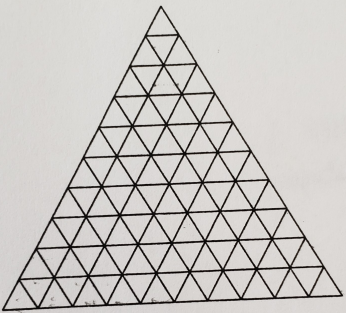
\includegraphics[scale=0.1]{TRIANGLE22.jpg}
\centering
\end{figure}
\begin{solution}
There can be three orientations of parallelograms, shown below, which by symmetry must have the same number of parallelograms. Thus, we can count one and multiply that number by three.
\begin{figure}[H]
% 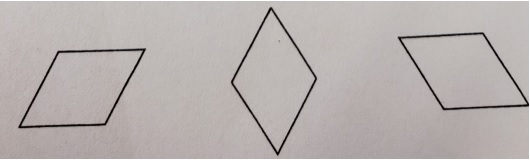
\includegraphics[scale=0.1]{TRIANGLE23.jpg}
\centering
\end{figure}
We can observe that a parallelograms has four lines that can be extended out. If we extend them out to one layer lower than the triangle, we can notice that the lines intersect with the bottom layer to find four points. Each one of the parallelograms corresponds to a unique selection of the four points, and vice versa.
\begin{figure}[H]
% 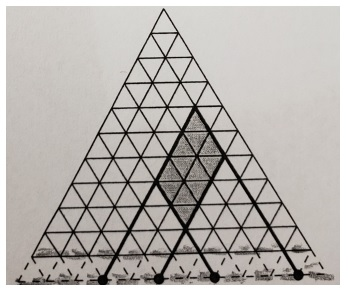
\includegraphics[scale=0.1]{TRIANGLE24.jpg}
\centering
\end{figure}
Thus, for each of the $n+2$ points on the level below the last one, we can choose four of them to get a unique parallelogram. Thus, in conclusion, the solution is \[3\cdot{n+2 \choose 4}\]
\end{solution}
\subsection{Hat Problem}
\begin{problem}
	2 n mathematicians walk into a bar. They each remove their hat and toss it in a pile as they arrive. Several hours later, they leave one by one, grabbing a hat at random to face the brutal March wind. What is the probability that none of the mathematicians receive their own hat?
\end{problem}
\begin{solution}
	This problem is equivalent to finding the number of \textbf{Derangement} of a set of size n, up to a factor of $n!$. The derangement number is notated as $D_n,$ or $!n.$
	\newline
	We can approach this by counting the number of ways to get the desired outcome via complementary counting, and then to divide it through by the total number of arrangements to get the probability, as each configuration is equally likely. First, to count the number of ways in total that there can be reordered. This is just n!. However, in this, we have counted the number of ways that at least $0$ mathematicians receive their hat. Next, we must subtract out the cases that have at least $1$ mathematician getting back his or her hat. We can count this by choosing which mathematician gets his or her hat back, and then ordering the rest. Thus, the term is ${n\choose1}\left(n-1\right)!.$ However, this overcounts those configurations for which more than one mathematician receives their hat back; we can fix this problem by using the principle of inclusion/exclusion, to get that the total number of derangements is \[n!-{n\choose1}\left(n-1\right)!+{n\choose2}\left(n-2\right)!+\cdots+(-1)^n{n\choose n}\left(n-n\right)!.\]
	This approaches $\frac{n!}{e}$ for sufficiently large $n$, as $e^x=1+x+x^2/2!+\cdots.$ Thus, by dividing the nth derangement number by $n!,$ we get the probability to be \[1-\frac{1}{1!}+\frac{1}{2!}+\cdots+\frac{(-1)^n}{n!}\approx e^{-1}\] for sufficiently large n.
\end{solution}
\subsection{"Coupon Collector"-esqe Problem}
\begin{problem}
	3 You have a bag containing $x$ numbered marbles. Draw $n$ marbles with replacement, where $n\leq x$. What is the probability that you drew exactly $k$ distinct marbles?
\end{problem}
\begin{solution}
To solve this, we can consider sequences of draws. First, we must determine the total number of "events" or valid sequences. There are $x^n$ such sequences. Next, we must pick $k$ of the $x$ distinct marbles to be seen, introducing a factor of ${x\choose k}.$ Next, we must partition the sequence of $n$ draws into $k$ subsets, each subset representing the draws that got one distinct value of the marble, introducing a factor of $S(n,k)$. And finally, we must assign each marble to a subset, introducing a factor of $k!.$ Thus, the probability is \[\frac{k!{x \choose n}S(n,k)}{x^n}.\]
\begin{example}
		If there are $10$ distinct marbles, we Draw $6$, and see $3$, one possible outcome is, if the number $j$ represent the $jth$ draw, \[C:\{1,4\},A:\{2,3,5\},B:\{6\}\]
		
\end{example}
Simplifying the probability a small amount, we get it to be \[\frac{x\fallingfactorial{k}S(n,k)}{x^n}.\]
This also turns out to be a way to prove that $x^n=\sum_{k=1}^{n}x\fallingfactorial{k}S(n,k),$ as the sum of the probabilities of all valid outcomes must be one.
\end{solution}
% \end{document}


\newpage 

\part{Generating Functions}
% %%%%%%% Lecture Notes Style for Concrete Mathematics %%%%%%%%%%%%%
%%%%%%% Taught by Patrick White, TJHSST %%%%%%%%%%%%%%%%%%%%%%%%%%

\documentclass[11pt,twosided]{article}
%%%%%%%%%%%%%%%%%%%%%%%%%%%%%%%%%%%%%%%%%%%%%%%%%%%%%%%
%%%% HEADER FILE for CONCRETE MATH LECTURE NOTES %%%%%%
%%%%%%%%%%%%%%%%%%%%%%%%%%%%%%%%%%%%%%%%%%%%%%%%%%%%%%%

%%%%%%%%%%%%%%%%%%%%%%%%%%%%%%%%%%%%%%%%%%%%%%%%%%%%%%%%%%%%%%%%%%%
%% This file is included at the top of every lecture notes file %%%
%% It should ONLY be changed by the instructor %%
%%%%%%%%%%%%%%%%%%%%%%%%%%%%%%%%%%%%%%%%%%%%%%%%%%%%%%%%%%%%%%%%%%%

%%%%%%%%%%%%%%%%%%%%%% package inclusions %%%%%%%%%%%%%%%%%%%%
%\usepackage[
%top=2cm,
%bottom=2cm,
%left=3cm,
%right=2cm,
%headheight=17pt, % as per the warning by fancyhdr
%includehead,includefoot,
%heightrounded, % to avoid spurious underfull messages
%]{geometry} 


\usepackage{amsmath,amssymb,amsfonts}
\usepackage{longtable}
\usepackage{mathtools}
\usepackage{amsthm}
\usepackage{enumerate}
\usepackage{fancyhdr}
\pagestyle{fancy}


%%%%%%%%%%%%%%% theorem style definitions %%%%%%%%%%%%%%%%%%%%%%
\newtheorem{theorem}{Theorem}[section]
%\newtheorem{corollary}{Corollary}[theorem]
%\newtheorem{lemma}[theorem]{Lemma}
\newtheorem*{remark}{Remark}
%\newtheorem{example}{Example}[section]
\newtheorem*{definition}{Definition}


%%%%%%%%%%%%%%%% custom function definitions %%%%%%%%%%%%%%%%%%%%%%%%%
%%%%%%%%%%% as class progresses, this section may be enhanced %%%%%%%%

\def\multiset#1#2{\ensuremath{\left(\kern-.3em\left(\genfrac{}{}{0pt}{}{#1}{#2}\right)
		\kern-.3em\right)}} %%% multiset notation
\newcommand\rf[2]{{#1}^{\overline{#2}}} %%%% rising factorial \rf{x}{m}
\newcommand\ff[2]{{#1}^{\underline{#2}}} %%%%% falling factorial \ff{x}{m}
\newcommand{\Perm}[2]{{}^{#1}\!P_{#2}} % permutation
\newcommand{\half}{\ensuremath{\frac{1}{2}}}
\newcommand{\braces}[1]{\left\{#1\right\}}
\newcommand{\set}[1]{\braces{#1}}
\newcommand{\snb}[2]{\ensuremath{\left(\kern-.3em\left(\genfrac{}{}{0pt}{}{#1}{#2}\right)\kern-.3em\right)}}
\newcommand{\fallingfactorial}[1]{^{\underline{#1}}}
\newcommand{\fallfac}[2]{{#1}^{\underline{#2}}}
\newcommand{\stirlingone}[2]{\genfrac[]{0pt}{1}{#1}{#2}}
\newcommand{\stiri}[2]{\stirlingone{#1}{#2}}
\newcommand{\dstirlingone}[2]{\genfrac[]{0pt}{0}{#1}{#2}}
\newcommand{\dstiri}[2]{\dstirlingone{#1}{#2}}
\newcommand{\stirlingtwo}[2]{\genfrac\{\}{0pt}{1}{#1}{#2}}
\newcommand{\stirii}[2]{\stirlingtwo{#1}{#2}}
\newcommand{\dstirlingtwo}[2]{\genfrac\{\}{0pt}{0}{#1}{#2}}
\newcommand{\dstirii}[2]{\dstirlingtwo{#1}{#2}}
\newcommand{\ol}[1]{\overline{#1}}
%%%%%%%
% book stuff
%%%%%%%%%

\usepackage[twoside,outer=1.5in,inner=2in,bottom=1.5in,top=1.5in,marginpar=2in]{geometry} 
\usepackage{scrextend}
\usepackage{palatino}
\usepackage{multicol}
\usepackage{float}
\usepackage[hidelinks]{hyperref}
\usepackage[nameinlink, capitalise, noabbrev]{cleveref}
%\usepackage{background}
\usepackage{graphicx}
\usepackage{listliketab}

\usepackage{lipsum}
\usepackage{caption}
\usepackage{marginnote}

\reversemarginpar


\usepackage[dvipsnames]{xcolor}
\usepackage{amsthm}
\usepackage{shadethm}

\setlength{\parindent}{0pt}

\newcommand*\Note{%
	\marginnote[\textcolor{blue}{\raggedright{\LARGE ?}\ Note }]{}%
}
\newcommand*\Warn{%
	\marginnote[\textcolor{red}{\raggedright{\LARGE !}\ Warning }]{}%
}
\reversemarginpar

\newcommand{\N}{\mathbb{N}}
\newcommand{\Z}{\mathbb{Z}}
\newcommand{\I}{\mathbb{I}}
\newcommand{\R}{\mathbb{R}}
\newcommand{\Q}{\mathbb{Q}}
\renewcommand{\qed}{\hfill$\blacksquare$}
\let\newproof\proof
\renewenvironment{proof}{\begin{addmargin}[1em]{0em}\begin{newproof}}{\end{newproof}\end{addmargin}\qed}
% \newcommand{\expl}[1]{\text{\hfill[#1]}$}


\newenvironment{lemma}[2][Lemma]{\begin{trivlist}
		\item[\hskip \labelsep {\bfseries #1}\hskip \labelsep {\bfseries #2.}]}{\end{trivlist}}
\newenvironment{problem}[2][Problem]{\begin{trivlist}
		\item[\hskip \labelsep {\bfseries #1}\hskip \labelsep {\bfseries #2.}]}{\end{trivlist}}
\newenvironment{example}[2][Example]{\begin{trivlist}
		\item[\hskip \labelsep {\bfseries #1}\hskip \labelsep{\bfseries #2.}]}{\end{trivlist}}
\newenvironment{solution}{{\noindent \bfseries Solution\hskip 2ex}}{\qed}
\newenvironment{exercise}[2][Exercise]{\begin{trivlist}
		\item[\hskip \labelsep {\bfseries #1}\hskip \labelsep {\bfseries #2.}]}{\end{trivlist}}
\newenvironment{reflection}[2][Reflection]{\begin{trivlist}
		\item[\hskip \labelsep {\bfseries #1}\hskip \labelsep {\bfseries #2.}]}{\end{trivlist}}
\newenvironment{proposition}[2][Proposition]{\begin{trivlist}
		\item[\hskip \labelsep {\bfseries #1}\hskip \labelsep {\bfseries #2.}]}{\end{trivlist}}
\newenvironment{corollary}[2][Corollary]{\begin{trivlist}
		\item[\hskip \labelsep {\bfseries #1}\hskip \labelsep {\bfseries #2.}]}{\end{trivlist}}
%%%% add package inclusions here, if any

%%%%% Define your custom functions and macros here, if any

%%%%%%%%%%%%%%%%%%%% Define the variables below %%%%%%%%%%%%%%%%%%%%%%%%%%%%%%
\def\titlestring{Counting \& Generating Functions}
\def\scribestring{Anupama Jayaraman, Ritika Shrivastav}
\def\datestring{Monday, March, 4 2019}


%%%%%%%%%%%%%%%%%%% Page Headers -- Do Not Change %%%%%%%%%%%%%%%%%%%%%%%%%%%
\lhead{\titlestring}
\rhead{Page \thepage}
\cfoot{Concrete Math -- White -- TJHSST}
\renewcommand{\headrulewidth}{0.4pt}
\renewcommand{\footrulewidth}{0.4pt}

%%%%%%%%%%%%%%%%% Begin the document %%%%%%%%%%%%%%%%%%%%%%%%%
\begin{document}
\thispagestyle{plain}  %% no headers on this page

%%%% Do not change these lines %%%%%
\noindent
{\LARGE \textbf{\titlestring}}\\\\
%
{\Large Scribe: \scribestring}\\ \\
{\textbf{Date}: \datestring}


%%%%%%%%%%%%%%%%%%%%%%%%%% YOUR CONTENT GOES HERE %%%%%%%%%%%%%%%%%%%%%%%%%%
\noindent

\section{Unit One: Counting}

\begin{center} * \end{center}
\begin{center} *\space\space\space\space* \end{center}
\begin{center} *\space\space\space\space*\space\space\space\space* \end{center}
\begin{center} *\space\space\space\space*\space\space\space\space*\space\space\space\space* \end{center}
\begin{center} *\space\space\space\space*\space\space\space\space*\space\space\space\space*\space\space\space\space* \end{center}
\begin{center} *\space\space\space\space*\space\space\space\space*\space\space\space\space*\space\space\space\space*\space\space\space\space* \end{center}
\newline \newline

\begin{example}
    1 We want to find a different way of counting the number of parallelograms that can be made by connecting the stars in the arrangement above.
\end{example}
\begin{solution} 
    One method to do this would be to pick a diagonal. We can say that picking the diagonal is unique because only one parallelogram will have the certain segment as its longest diagonal. To determine the number of diagonals, we need to pick the number of line segments we can make using the points.\newline
    \newline
    This can be done by taking the total number of points and choosing 2. \newline
    For a triangle of $n$ rows, the number of points is $\frac{(n)(n+1)}{2}$ or ${n+1 \choose 2}$ \newline
    To choose two dots we do ${{n+1 \choose 2} \choose 2}$ \newline
    \newline 
    However, we have to remember that if two dots are on the same line, then they won't be able to form the longest diagonal of a parallelogram, and if both are on an edge, it wouldn't be relevant. Therefore, we have to subtract for the times when the two dots chosen are collinear. \newline
    \newline
    So the subtracted values would be $3* some value$ because we have three orientations of the triangle to account for. (Another way of looking at this would be to say that we have 3 sides of the triangle to account for).\newline
    Now, to determine "some value". We realize that some value in one orientation is actually just the same as counting for each row, how many ways they can pick two points. \newline
    \newline
    This can actually be written as a summation: $\sum_{i=2}^{n}{i \choose 2}$ \newline
    To explain, the sum. We know we must start at i=2, because a row with one dot cannot pick two dots that are collinear. We use the summation because in the i-th row there are i dots and we need to pick 2 of them. \newline
    \newline
    This therefore results in a final solution of ${{{n+1 \choose 2} \choose 2} - 3 * \sum_{i=2}^{n}{i \choose 2}}$ \newline
    \newline
    After some algebra, our final answer is
    \fbox{$3$${n+1 \choose 4}$}
\end{solution}    


\section{Unit Two: Generating Functions}
\begin{problem}
    1 Find the $nth$ term in the sequence if the the first term corresponds with $n=0$:
     \begin{center} 1, 2, 4, 8, 16, ...\end{center}
      \end{problem}
\begin{solution}
$a_{0} = 1$, $a_{1} = 2$, $a_{2} = 4$. It is clear from this pattern that $a_{n} = 2^{n}$. 
\end{solution}

\begin{problem}
    2 Find the generating function for:
     \begin{center} 1, 2, 4, 8, 16, ...\end{center}
\end{problem}
\begin{solution}
In a generating function, the coefficients of each power correspond to each of the terms in the sequence. This sequence can thus be represented as $g(x) = 1*x^{0} + 2*x^{1} + 4*x^{2} + 8*x^{3} + 16*x^{4} + 32*x^{5} + ... = (2x)^0 + (2x)^1 + (2x)^2 + (2x)^3 + (2x)^4 + (2x)^5 + ...$. This resembles the the Taylor power series. Using 'reverse'-Taylor, we find that $g(x) = \frac{1}{1-2x}$. 
\end{solution} \\
 

\\From this example, we can see that $\frac{1}{1-ax}$ is the generating function for the sequence $1, a, a^2, a^3, ... = \{a^k\}_{k=0}$. Generally, from the generating function, to obtain the $nth$ value of the sequence, take the nth derivative of the function evaluated at 0.\newline

\begin{problem}
    3 For the following sequence, find the generating function:
    \begin{center} 2, 5, 13, 35, 97, ... \end{center}
\end{problem}

\begin{solution}
The $nth$ term of the sequence is $a_{n} = 2^{n} + 3^{n}$. From above, we know that $\frac{1}{1-2x}$ generates $\{2^n\}$ and $\frac{1}{1-3x}$ generates $\{3^n\}$. Since \textbf{we can add generating functions}, $\frac{1}{1-2x}+\frac{1}{1-3x}$ generates $\{2^n +3^n\}$. If we simplify, we get the generating function $g(x)=\frac{2-5x}{1-5x+6x^2}$.
\end{solution}

\begin{problem}
4 Given the Fibonacci sequence, find the generating function. Then find the non-recursive definition of the $nth$ term: 
\begin{center} $f_{0}=0, f_{1}=1, f_{n}=f_{n-1}+f_{n-2}$ \end{center}
\begin{center} 0, 1, 1, 2, 3, 5, 8, 13, 21, ... \end{center}
\end{problem}

\begin{solution} \\
Finding the generating function: \\To find the function $F(x)$, we need to reduce the number of terms we are dealing with. $F(x) = x + x^2 + 2x^3 + 3x^4 + 5x^5 + ...$. We can see that the coefficient of the $x^3$ term is the sum of the coefficients of the $x^2$ and $x$ terms, as per the definition of the sequence. To cancel out the terms, let's shift the the function by ${x}$ and ${x^2}$.\\
$F(x) = x + x^2 + 2x^3 + 3x^4 + 5x^5 + ...$\\
$x * F(x) = x^2 + x^3 + 2x^4 + 3x^5 + ...$ \\
$x^2*F(x) = \indent   x^3 + x^4 + 2x^5 + ...$ \\
By subtracting, we get $(1-x-x^2)*F(x) = x$, or $F(x) = \frac{x}{1-x-x^2}$. \\ \\ 
Finding the non-recursive definition: \\By partial fraction decomposition, we can break down $F(x)$ into the form of $\frac{A}{1-\alpha x}+\frac{b}{1-\beta x}$. This corresponds with the form $F_{n}=A*\alpha ^n + B*\beta ^n$. After solving for $A, B, \alpha,$ and $\beta$, we find that $F_{n}=\frac{1}{\sqrt{5}}[(\frac{1+\sqrt{5}}{2})^{n} - (\frac{1-\sqrt{5}}{2})^{n}]$.
\end{solution}


\end{document}


\part{Groups and Group Actions}

\part{Coda: Computational Complexity}


\end{document} 
